\documentclass[10pt,twocolumn,letterpaper]{article}

\usepackage{cvpr}
\usepackage{times}
\usepackage{epsfig}
\usepackage{graphicx}
\usepackage{amsmath}
\usepackage{amssymb}

%%%%%%%%%%%%%%%%%%%%%%%%%%%%%%%%%%%%%%%%%%%%%%%%%%%%%%%%%

\usepackage{mathtools}
\usepackage{acronym}
\usepackage{caption}
\usepackage{array}
\usepackage{tabularx}
\usepackage{subcaption}
\usepackage{booktabs}
\usepackage{multicol}
\usepackage{multirow}

%%%%%%%%%%%%%%%%%%%%MACROS%%%%%%%%%%%%%%%%%%%%%%%%%%%
% acronyms
% \acrodef{SEAN}{Semantic (Region)-Adaptive Normalization}

\acrodef{SPADE}{Spatially-Adaptive Normalization}
\acrodef{AdaIN}{Adaptive Instance Normalization}
\acrodef{LRN}{Local Response Normalization}
\acrodef{BN}{Batch Normalization}
\acrodef{IN}{Instance Normalization}
\acrodef{LN}{Layer Normalization}
\acrodef{GN}{Group Normalization}
\acrodef{WN}{Weight Normalization}
\acrodef{Conditional BN}{Conditional Batch Normalization}

\acrodef{mIoU}{mean Intersection-over-Union}
\acrodef{accu}{pixel accuracy}
\acrodef{FID}{Fréchet Inception Distance}


\def\facade{fa\c{c}ade\xspace}
\def\facades{fa\c{c}ades\xspace}
\def\Facade{Fa\c{c}ade\xspace}
\def\Facades{Fa\c{c}ades\xspace}

\newcommand{\todo}{{\textbf{\color{red}[TO-DO]\_}}}



% Include other packages here, before hyperref.

% If you comment hyperref and then uncomment it, you should delete
% egpaper.aux before re-running latex.  (Or just hit 'q' on the first latex
% run, let it finish, and you should be clear).
\usepackage[pagebackref=true,breaklinks=true,letterpaper=true,colorlinks,bookmarks=false]{hyperref}

\cvprfinalcopy % *** Uncomment this line for the final submission

\def\cvprPaperID{} % *** Enter the CVPR Paper ID here
\def\httilde{\mbox{\tt\raisebox{-.5ex}{\symbol{126}}}}

% Pages are numbered in submission mode, and unnumbered in camera-ready
\pagestyle{empty}

\begin{document}

%%%%%%%%% TITLE
\title{SEAN: Image Synthesis with Semantic Region-Adaptive Normalization}

\author{Peihao Zhu\textsuperscript{1} \quad Rameen Abdal\textsuperscript{1} \quad Yipeng Qin\textsuperscript{2} \quad Peter Wonka\textsuperscript{1} \\
\\
\textsuperscript{1}KAUST \quad \textsuperscript{2}Cardiff University
}

% \author{
% Pei-Hao Zhu\\
% KAUST\\
% {\tt\small peihao.zhu@kaust.edu.sa}
% % For a paper whose authors are all at the same institution,
% % omit the following lines up until the closing ``}''.
% % Additional authors and addresses can be added with ``\and'',
% % just like the second author.
% % To save space, use either the email address or home page, not both
% \and
% Rameen Abdal\\
% KAUST\\
% {\tt\small rameen.abdal@kaust.edu.sa}
% \and
% Yipeng Qin\\
% Cardiff University\\
% {\tt\small qiny16@cardiff.ac.uk}
% \and
% Peter Wonka\\
% KAUST\\
% {\tt\small pwonka@gmail.com}
% }



\maketitle
\thispagestyle{empty}
\appendix

%%%%%%%%% ABSTRACT
\section{Additional Implementation Details}

\noindent {\bf Generator.} Our generator consists of several SEAN ResBlks. Each of them is followed by a nearest neighbor upsampling layer. Note that we only inject the style codes $\mathbf{ST}$ into the first 6 SEAN ResBlks. The other inputs are injected to all SEAN ResBlks. The architecture of our generator is shown in Figure~\ref{fig:SEAN generator architecture}.


\begin{figure}[ht]
\centering
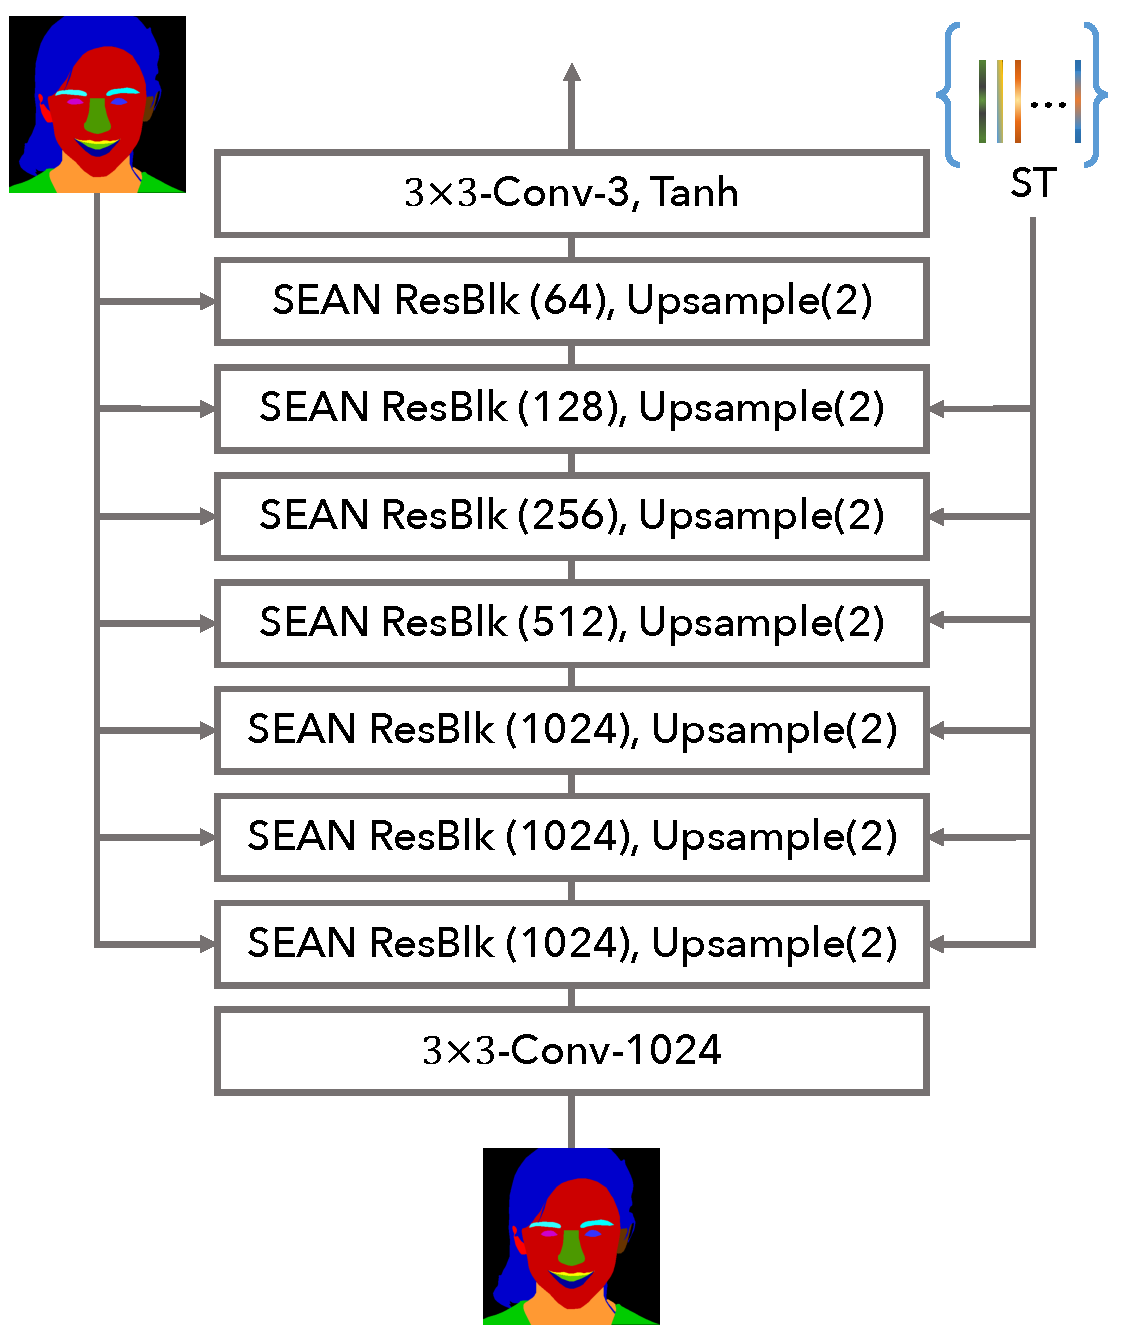
\includegraphics[width=0.9\linewidth]{Supp/architecture/supp_generator.pdf}
\caption{SEAN Generator. The style codes $\mathbf{ST}$ and segmentation mask are passed to the generator through the proposed SEAN ResBlks. The number of feature map channels is shown in the parenthesis after each SEAN ResBlk. To better illustrate the architecture, we omit the learnable noise inputs and per-style Conv layers in this figure. These details are shown in Fig.3 of the main paper (see $A_{ij}$ and $B_{ij}$).}
\label{fig:SEAN generator architecture}
\end{figure}


\noindent {\bf Discriminator.} Following SPADE~\cite{park2019SPADE} and Pix2PixHD~\cite{wang2018pix2pixHD}, we employed two multi-scale discriminators with instance normalization (IN)~\cite{ulyanov2016instance} and Leaky ReLU (LReLU). Similar to SPADE, we apply spectral normalization~\cite{miyato2018spectral} to all the convolutional layers of the discriminator. The architecture of our discriminator is shown in Figure~\ref{fig:SEAN discriminator architecture}.
 

\begin{figure}[ht]
\centering
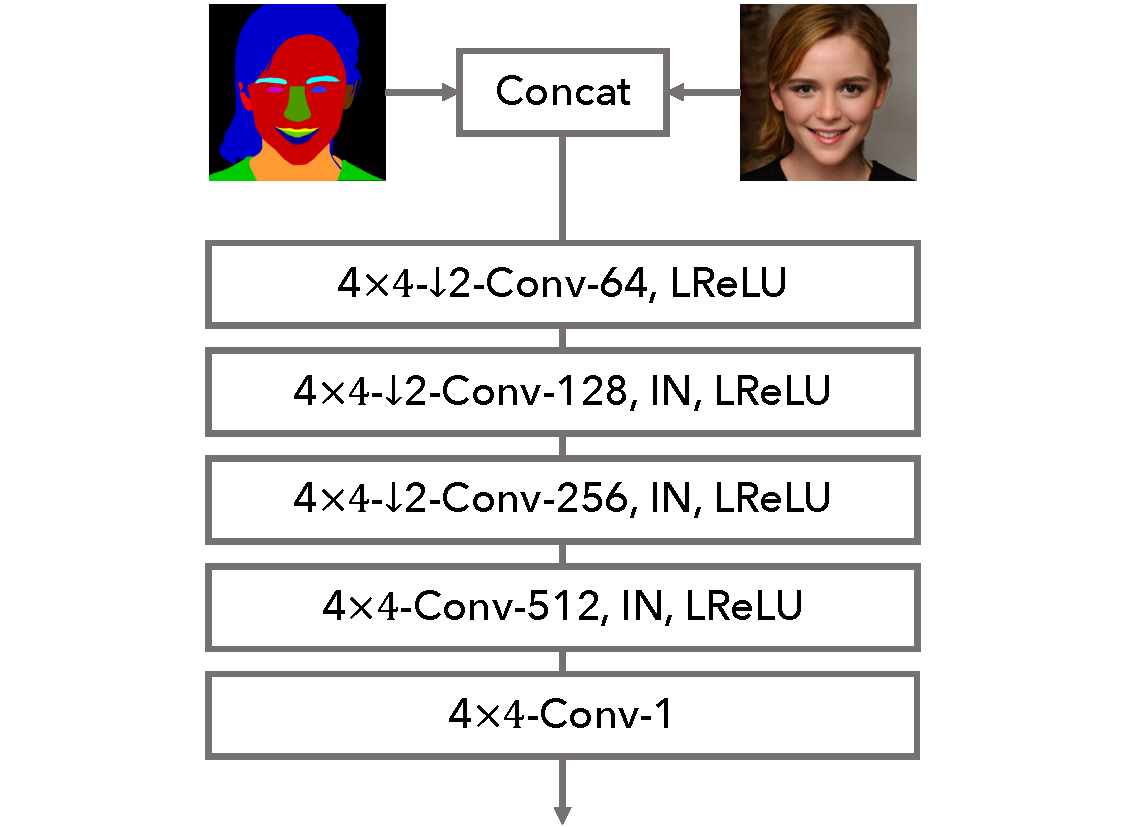
\includegraphics[width=0.9\linewidth]{Supp/architecture/supp_discriminator.pdf}
\caption{Following SPADE and Pix2PixHD, our discriminator takes the concatenation of a segmentation mask and a style image as inputs. The loss is calculated in the same way  as PatchGAN~\cite{isola2016imagetoimage}.}
\label{fig:SEAN discriminator architecture}
\end{figure}

\noindent {\bf Style Encoder.} Our style encoder consists of a ``bottleneck'' convolutional neural network and a region-wise average pooling layer (Figure~\ref{fig:SEAN style encoder architecture}). The inputs are the style image and the corresponding segmentation mask, while the outputs are the style codes $\mathbf{ST}$.

\begin{figure*}[th]
\centering
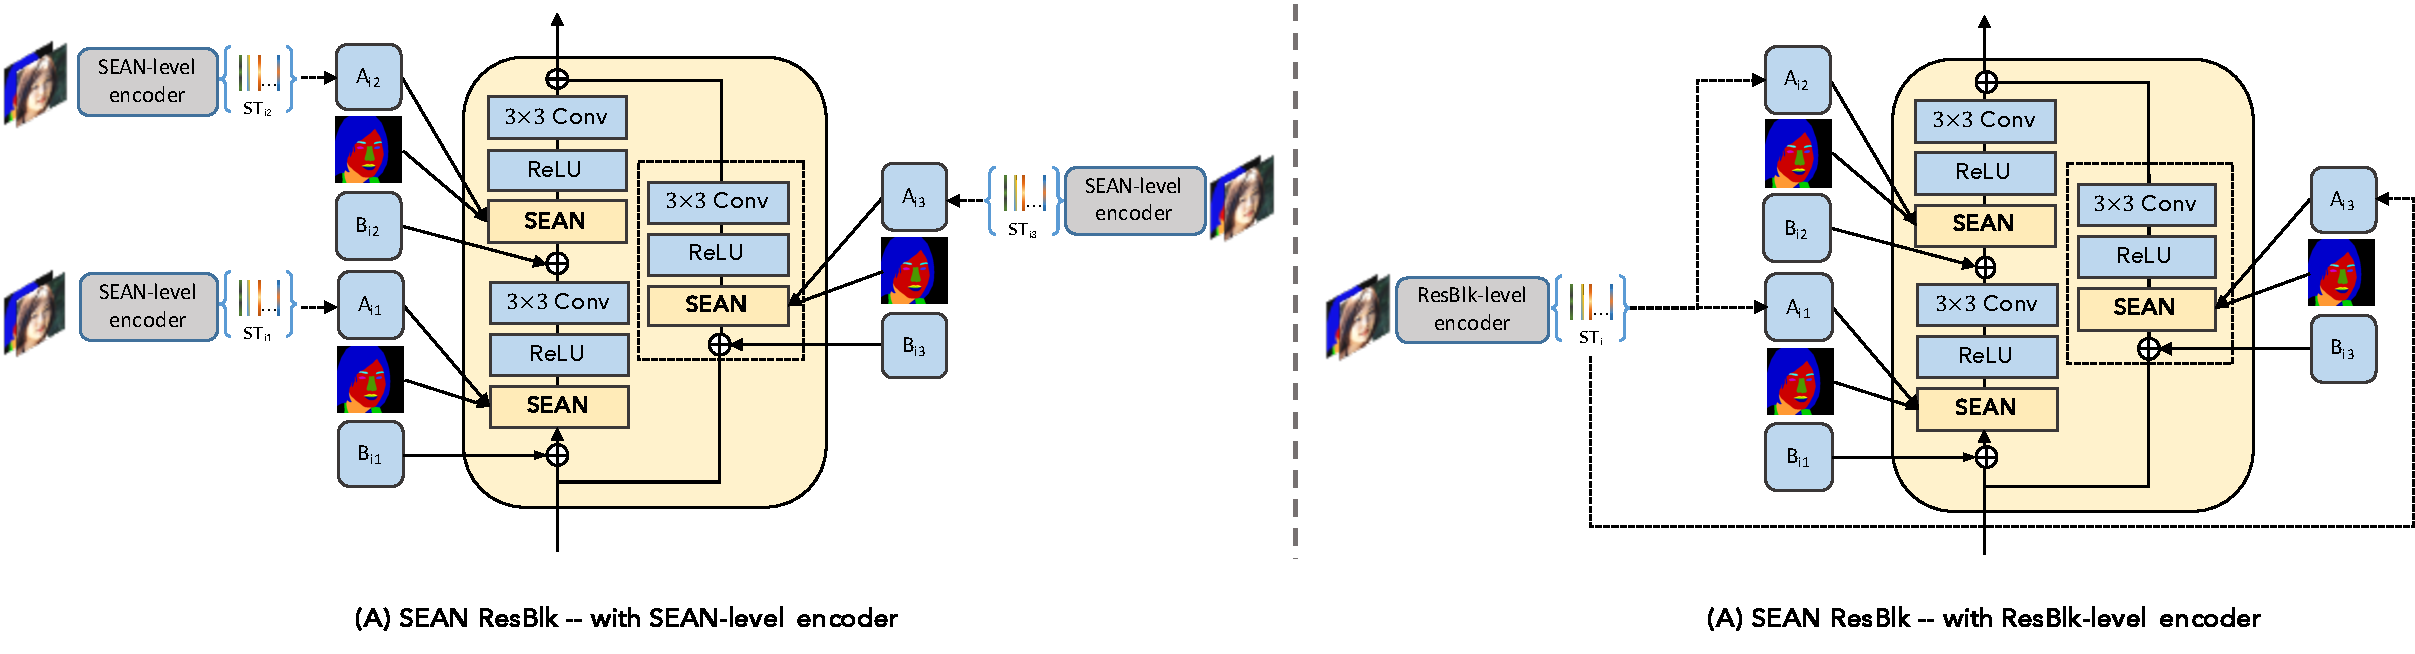
\includegraphics[width=\linewidth]{Supp/Different_encoders.pdf}
\caption{Detailed usage of the SEAN-level encoder and the ResBlk-level encoder within a SEAN ResBlk.}
\label{fig:different encoders}
\end{figure*}



\begin{figure}[ht]
\centering
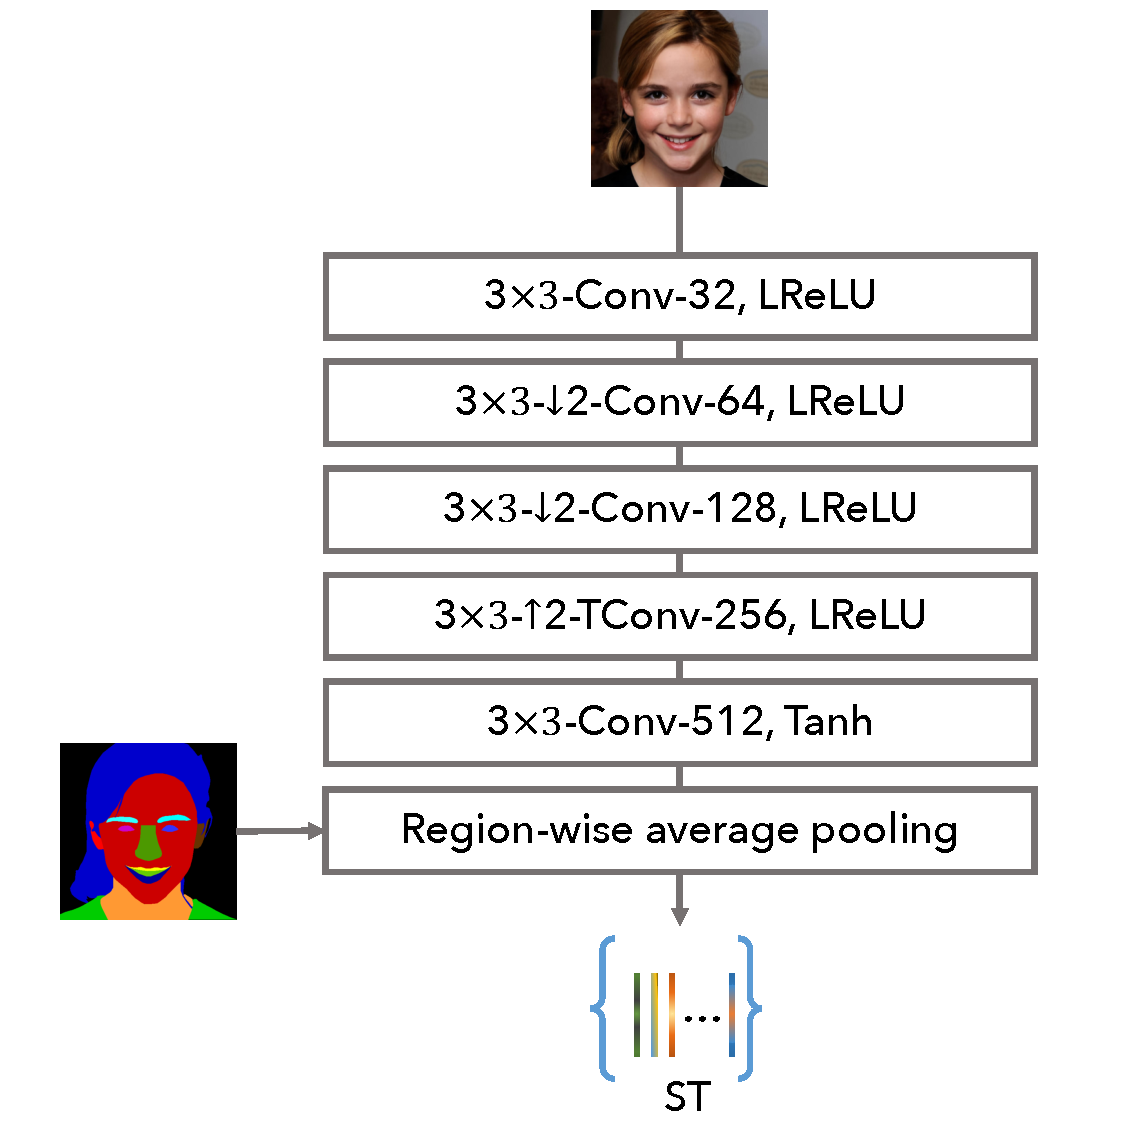
\includegraphics[width=0.9\linewidth]{Supp/architecture/supp_style_encoder.pdf}
\caption{Our style encoder takes the style image and the segmentation mask as inputs to generate the style codes $\mathbf{ST}$.}
\label{fig:SEAN style encoder architecture}
\end{figure}


\vspace*{3mm}\noindent {\bf Loss function.} The design of our loss function is inspired by those of SPADE and Pix2PixHD which contains three components:\\
 
\noindent (1) \textit{Adversarial loss.}
Let $E$ be the style encoder, $G$ be the SEAN generator, $D_1$ and $D_2$ be two discriminators at different scales~\cite{wang2018pix2pixHD}, $\mathbf{R}$ be a given style image, $\mathbf{M}$ be the corresponding segmentation mask of $\mathbf{R}$, we formulate the conditional adversarial learning part of our loss function as:
\small
\begin{equation}
\min _{E, G} \max _{D_{1}, D_{2}} \sum_{k=1,2} \mathcal{L}_{\mathrm{GAN}}\left(E, G, D_{k}\right)
\end{equation}
\normalsize
Specifically, $\mathcal{L}_{\mathrm{GAN}}$ is built with the Hinge loss that:
\small
\begin{equation}
\begin{split}
\mathcal{L}_{\mathrm{GAN}} &= \mathbb{E}\left[\max(0, 1-D_{k}(\mathbf{R, M}))\right] \\
&+  \mathbb{E}\left[\max(0, 1+D_{k}(G\mathbf{\left(\mathbf{ST,M}\right),M}))\right]
\label{eq:adversarial loss function}
\end{split}
\end{equation}
\normalsize
where $\mathbf{ST}$ is the style codes of $\mathbf{R}$ extracted by $E$ under the guidance of $\mathbf{M}$:
\small
\begin{equation}
\mathbf{ST} = E\left(\mathbf{R, M}\right)
\label{eq:ST function}
\end{equation}
\normalsize

\noindent (2) \textit{Feature matching loss}~\cite{wang2018pix2pixHD}. Let $T$ be the total number of layers in discriminator $D_{k}$, $D_{k}^{(i)}$ and $N_{i}$ be the output feature maps and the number of elements of the $i$-th layer of $D_{k}$ respectively, we denote the feature matching loss term $\mathcal{L}_{FM}$ as:

\small
\begin{equation}
\mathcal{L}_{FM}=\mathbb{E} \sum_{i=1}^{T}\frac{1}{N_{i}}\left[\left\|D_{k}^{(i)}(\mathbf{R} ,\mathbf{M})-D_{k}^{(i)}\left(G\mathbf{(ST,M)},\mathbf{M}\right)\right\|_{1}\right]
\label{eq:feature matching loss function}
\end{equation}
\normalsize

\noindent (3) \textit{Perceptual loss}~\cite{johnson2016perceptual}. Let $N$ be the total number of layers used to calculate the perceptual loss, $F^{(i)}$ be the output feature maps of the $i$-th layer of the VGG network~\cite{simonyan2014deep}, $M_{i}$ be the number of elements of $F^{(i)}$, we denote the perceptual loss $\mathcal{L}_{p e r c e p t}$ as:
\small
\begin{equation}
\mathcal{L}_{p e r c e p t}=\mathbb{E}\sum_{i=1}^{N} \frac{1}{M_{i}}\left[\left\|F^{(i)}\left(\mathbf{R}\right)-F^{(i)}\left(G\mathbf{(ST,M)}\right)\right\|_{1}\right]
\label{eq:perceptual loss function}
\end{equation}
\normalsize




The final loss function used in our experiment is made up of the above-mentioned three loss terms as: 
\small
\begin{equation}
\min_{E, G}\bigg( \Big( \max _{D_{1}, D_{2}} \sum_{k=1,2} \mathcal{L}_{\mathrm{GAN}} \Big) + \lambda_{1} \sum_{k=1,2} \mathcal{L}_{\mathrm{FM}} + \lambda_{2} \mathcal{L}_{\mathrm{p e r c e p t}}\bigg) 
\label{eq:overall loss}
\end{equation}
\normalsize
Following SPADE and Pix2PixHD, we set $\lambda_{1} = \lambda_{2} = 10$ in our experiments.




\vspace*{3mm}\noindent {\bf Training details.} We perform $50$ epochs of training on all the datasets mentioned in the main paper. During training, all input images are resized to a resolution of $256\times256$, except for the CityScapes dataset~\cite{Cordts2016Cityscapes} whose images are resized to $512\times256$. We use Glorot initialization~\cite{pmlr-v9-glorot10a} to initialize our network weights.

\section{Additional Experimental Details}


\noindent \textbf{Table 3 (main paper).}
Supplementing row 5 and 6 in Table 3 of the main paper, Figure~\ref{fig:different encoders} shows how the two variants of style encoders (\ie the SEAN-level encoder and the ResBlk-level encoder) are used in a SEAN ResBlk.
Specifically, the SEAN-level encoders extract different style codes for each SEAN block while the same style codes extracted by the ResBlk-level encoder are used by all SEAN blocks within a SEAN ResBlk. 
% while the unified encoder is the architecture described in the main part of the paper. 
% Although the first two encoders have better reconstruction performance, they lead to lower FID scores and worse style transfer performance as shown in Figure~\ref{fig:Encoder Comparison}. 



\vspace*{3mm}\noindent \textbf{Figure 6 (main paper).}
We used the Ground Truth (second column in Figure 6 of the main paper) as the style input for all methods.
For Pix2pixHD, we generate the results by: (i) encoding the style image into a style vector; (ii) broadcasting the style vector and concatenating it to the mask input of the generator. 


\section{Justification of Encoder Choice} Figure~\ref{fig:Encoder Comparison} shows that the images generated by the unified encoder are of better visual quality than those generated by the SEAN-level encoder, especially for challenging inputs (e.g. extreme poses, unlabeled regions), which justifies our choice of unified encoder. 


\addtolength{\tabcolsep}{-4.5pt}    
% \setlength{\mywidth}{0.1932\textwidth}
\bgroup
\def\arraystretch{0.5}%  1 is the default. Controls vertical spacing.
\begin{figure}[th]
\small
\begin{tabular} {cc|cc}
Label & Style Image & Encoder1 & Encoder2
\\
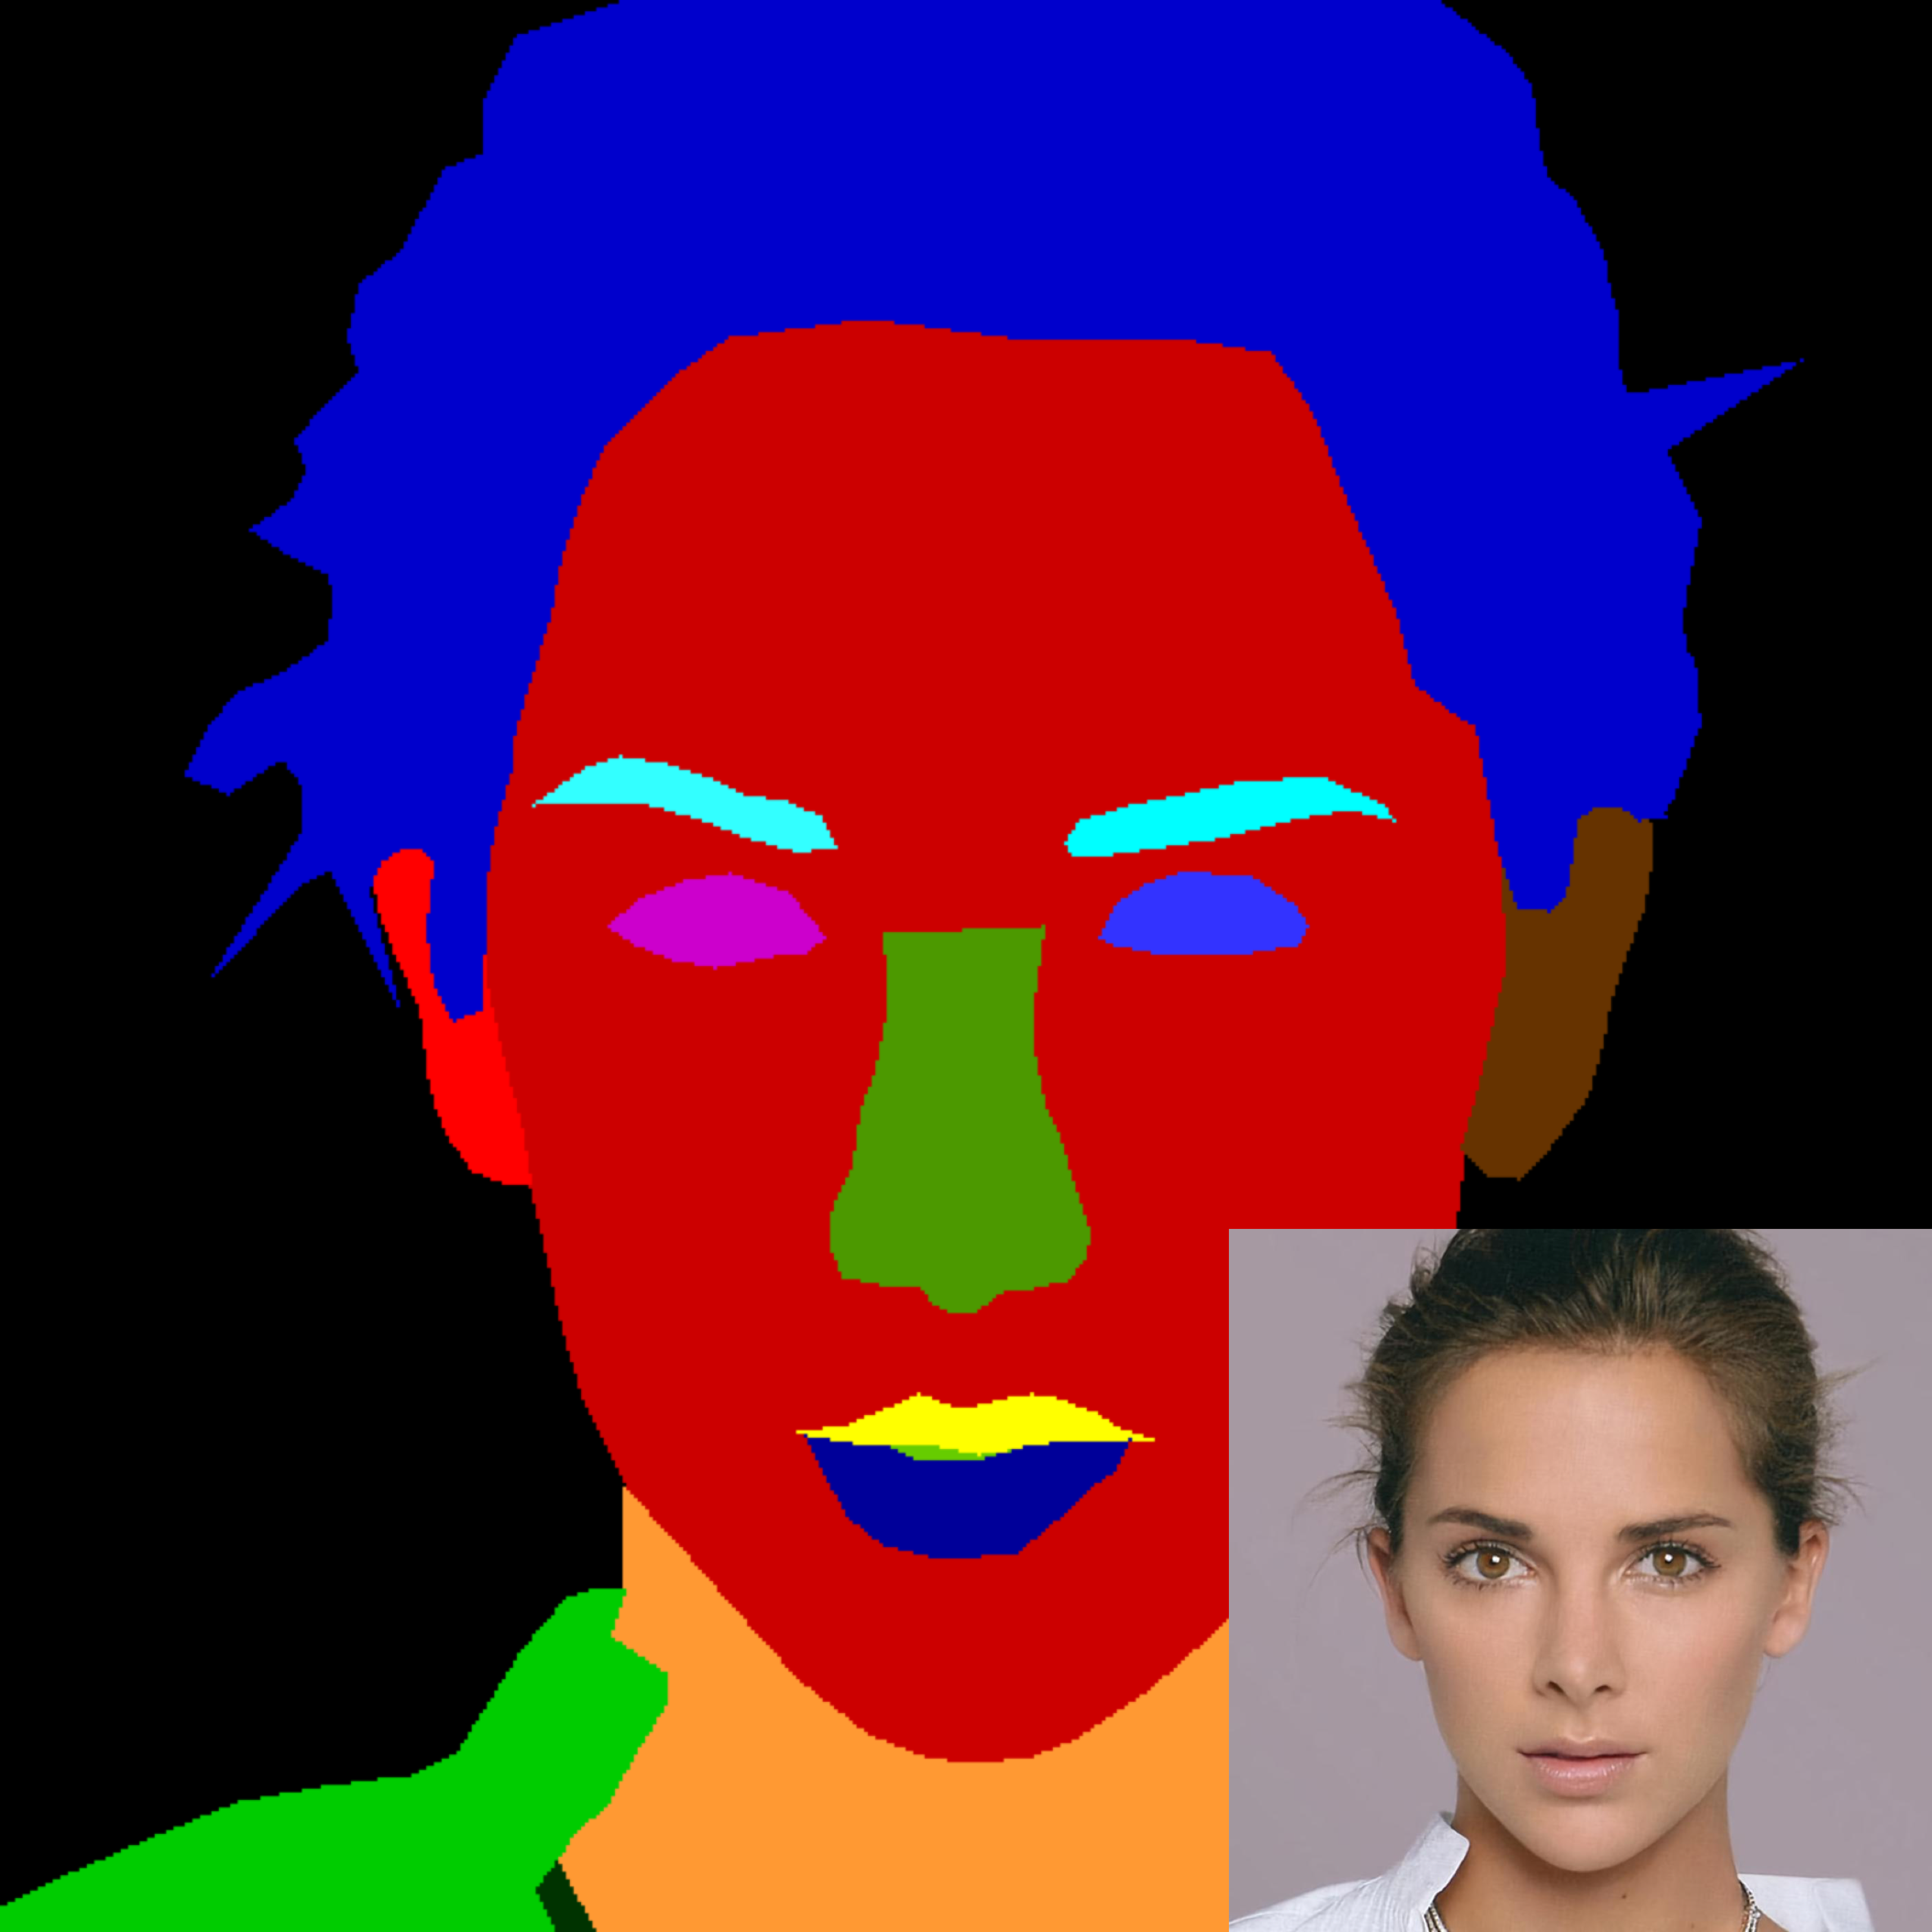
\includegraphics[width=0.11\textwidth]{Images/Encoder_search/encoder_1.png} & 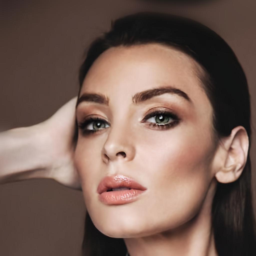
\includegraphics[width=0.11\textwidth]{Images/Encoder_search/style/29659.png} &
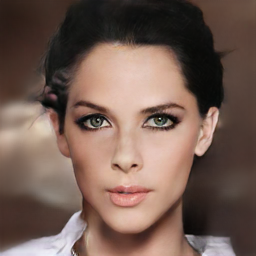
\includegraphics[width=0.11\textwidth]{Images/Encoder_search/SEAN_level/1.png} &   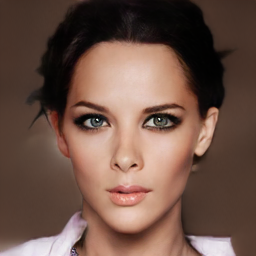
\includegraphics[width=0.11\textwidth]{Images/Encoder_search/Unified/1.png}\\ 

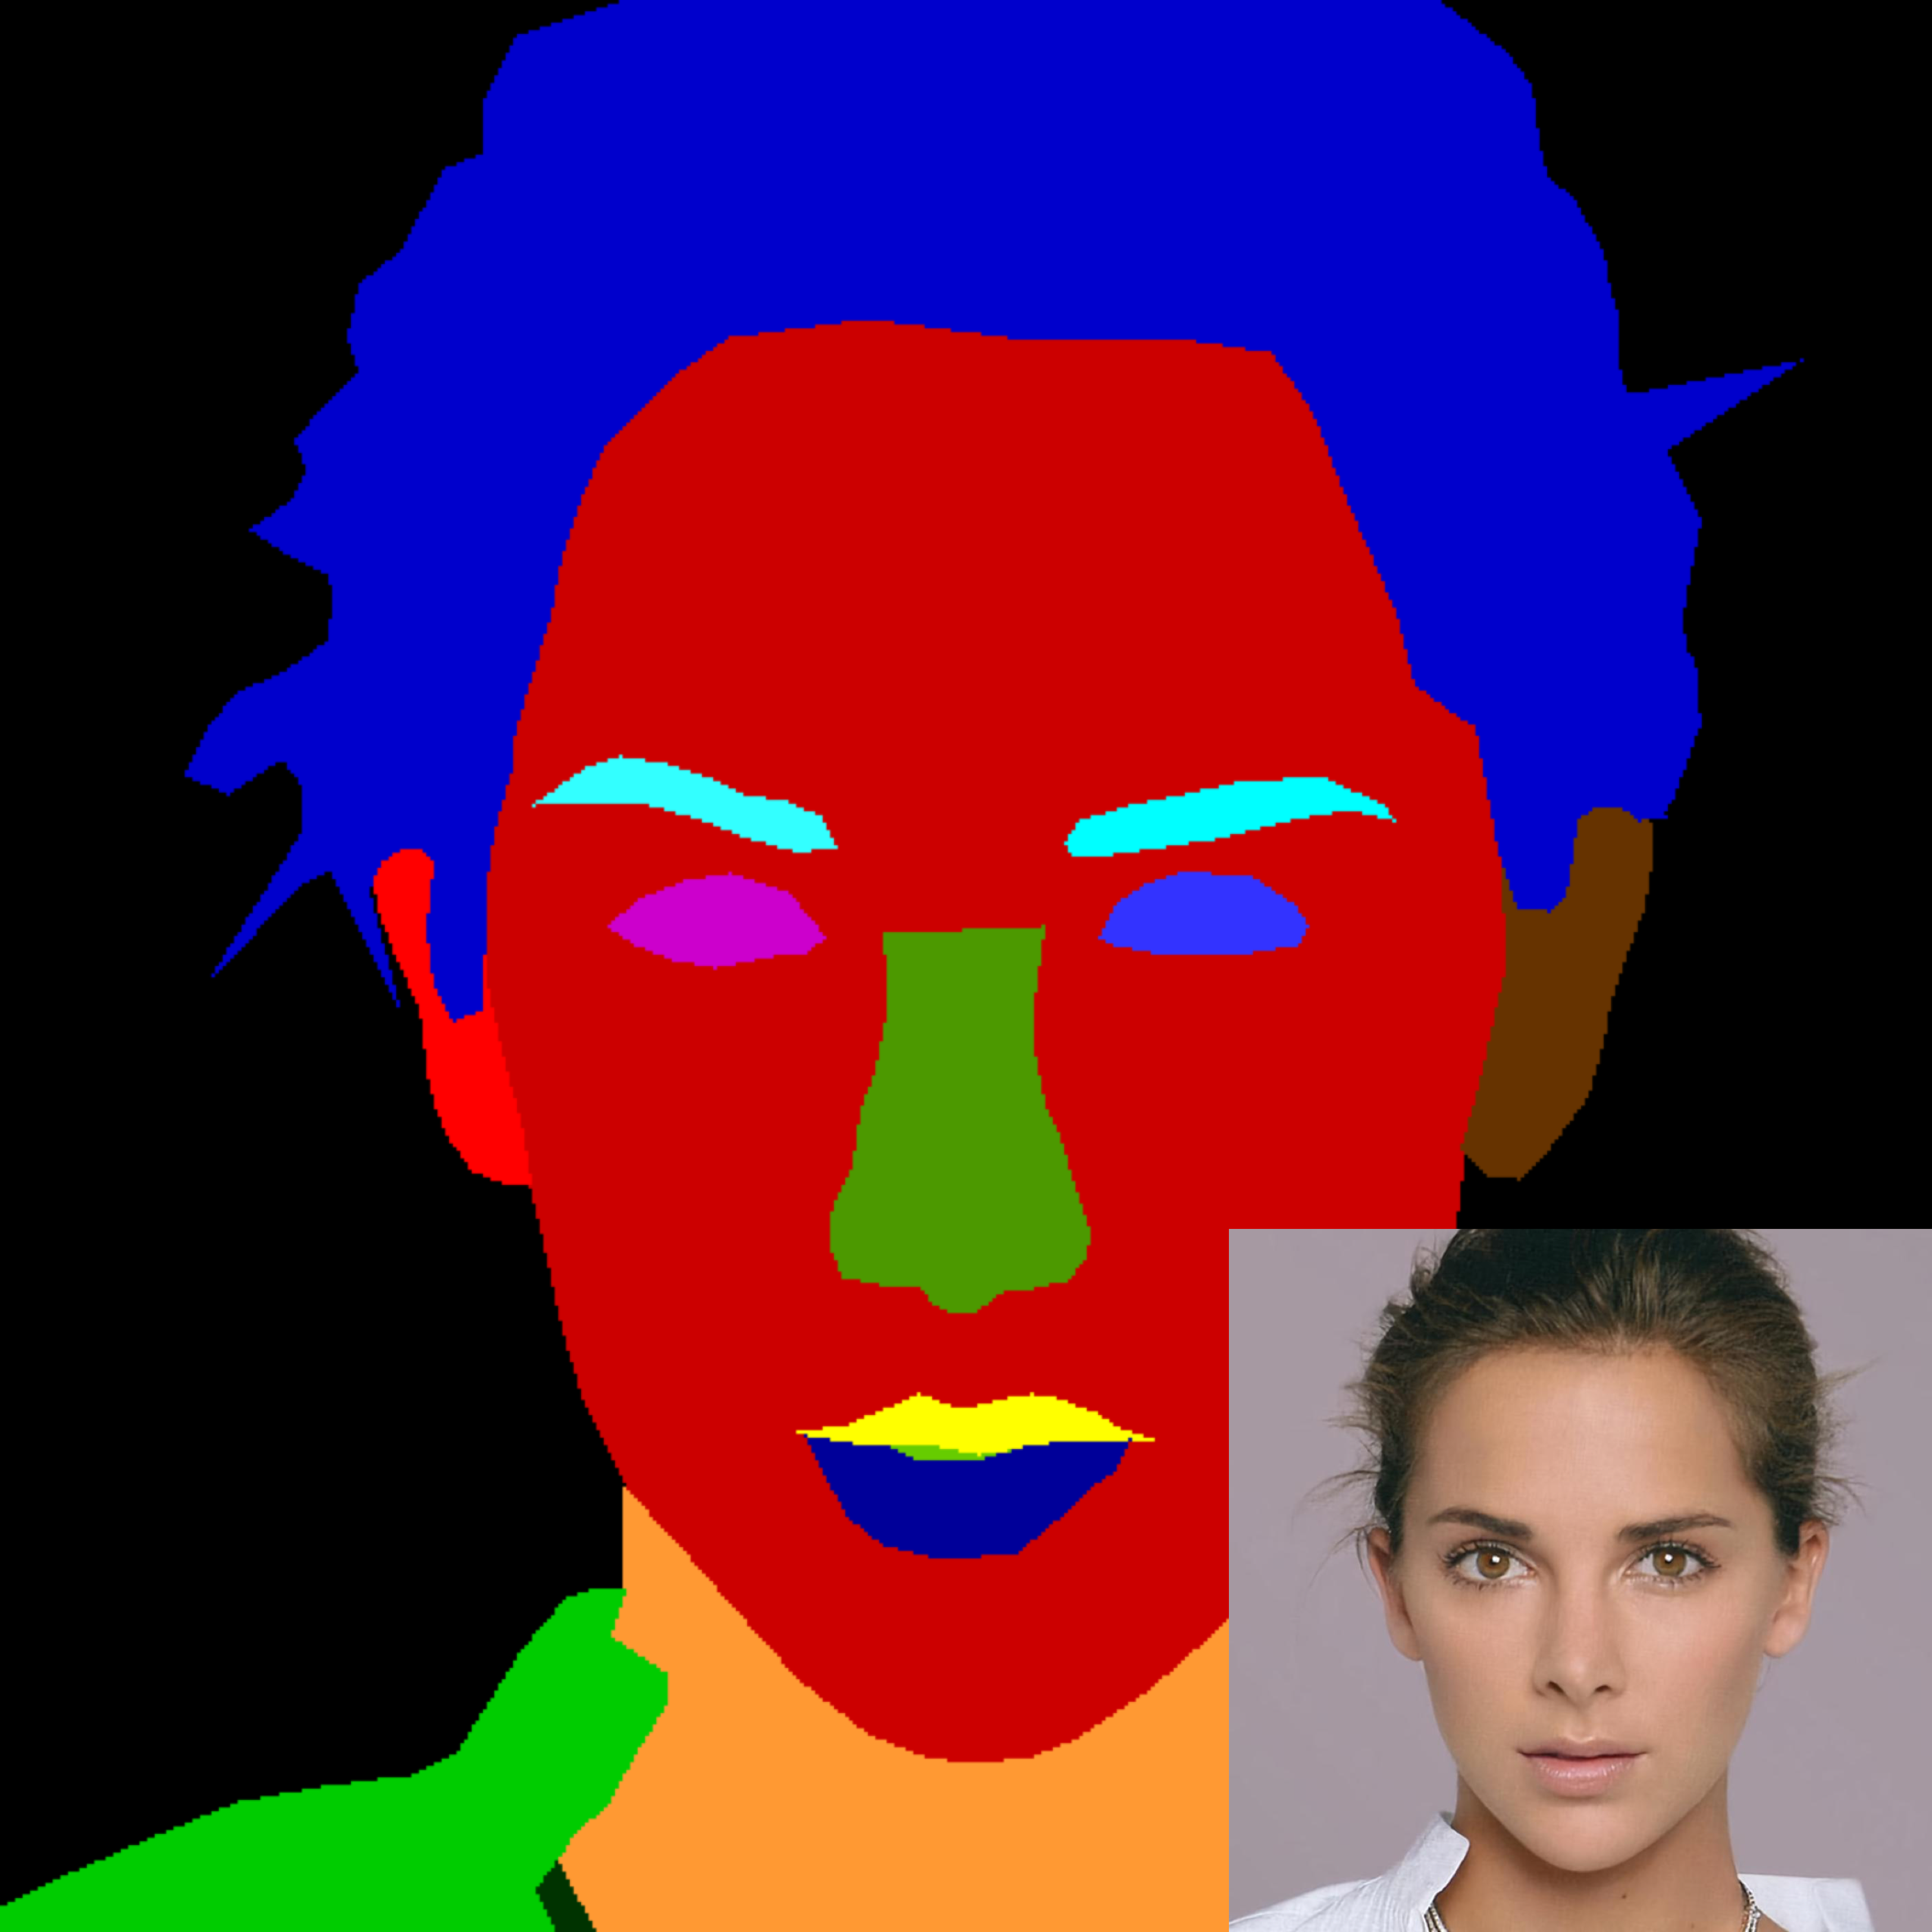
\includegraphics[width=0.11\textwidth]{Images/Encoder_search/encoder_1.png} & 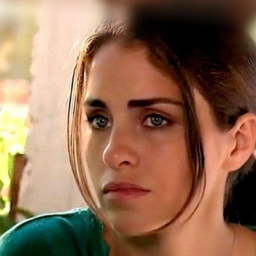
\includegraphics[width=0.11\textwidth]{Images/Encoder_search/style/29598.png} &
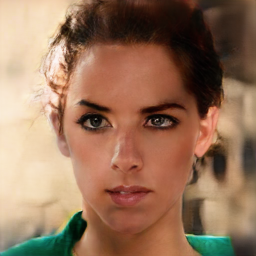
\includegraphics[width=0.11\textwidth]{Images/Encoder_search/SEAN_level/2.png} &   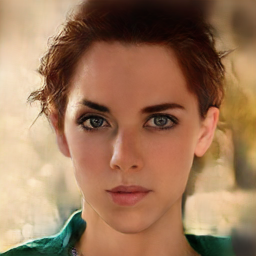
\includegraphics[width=0.11\textwidth]{Images/Encoder_search/Unified/2.png}\\ 

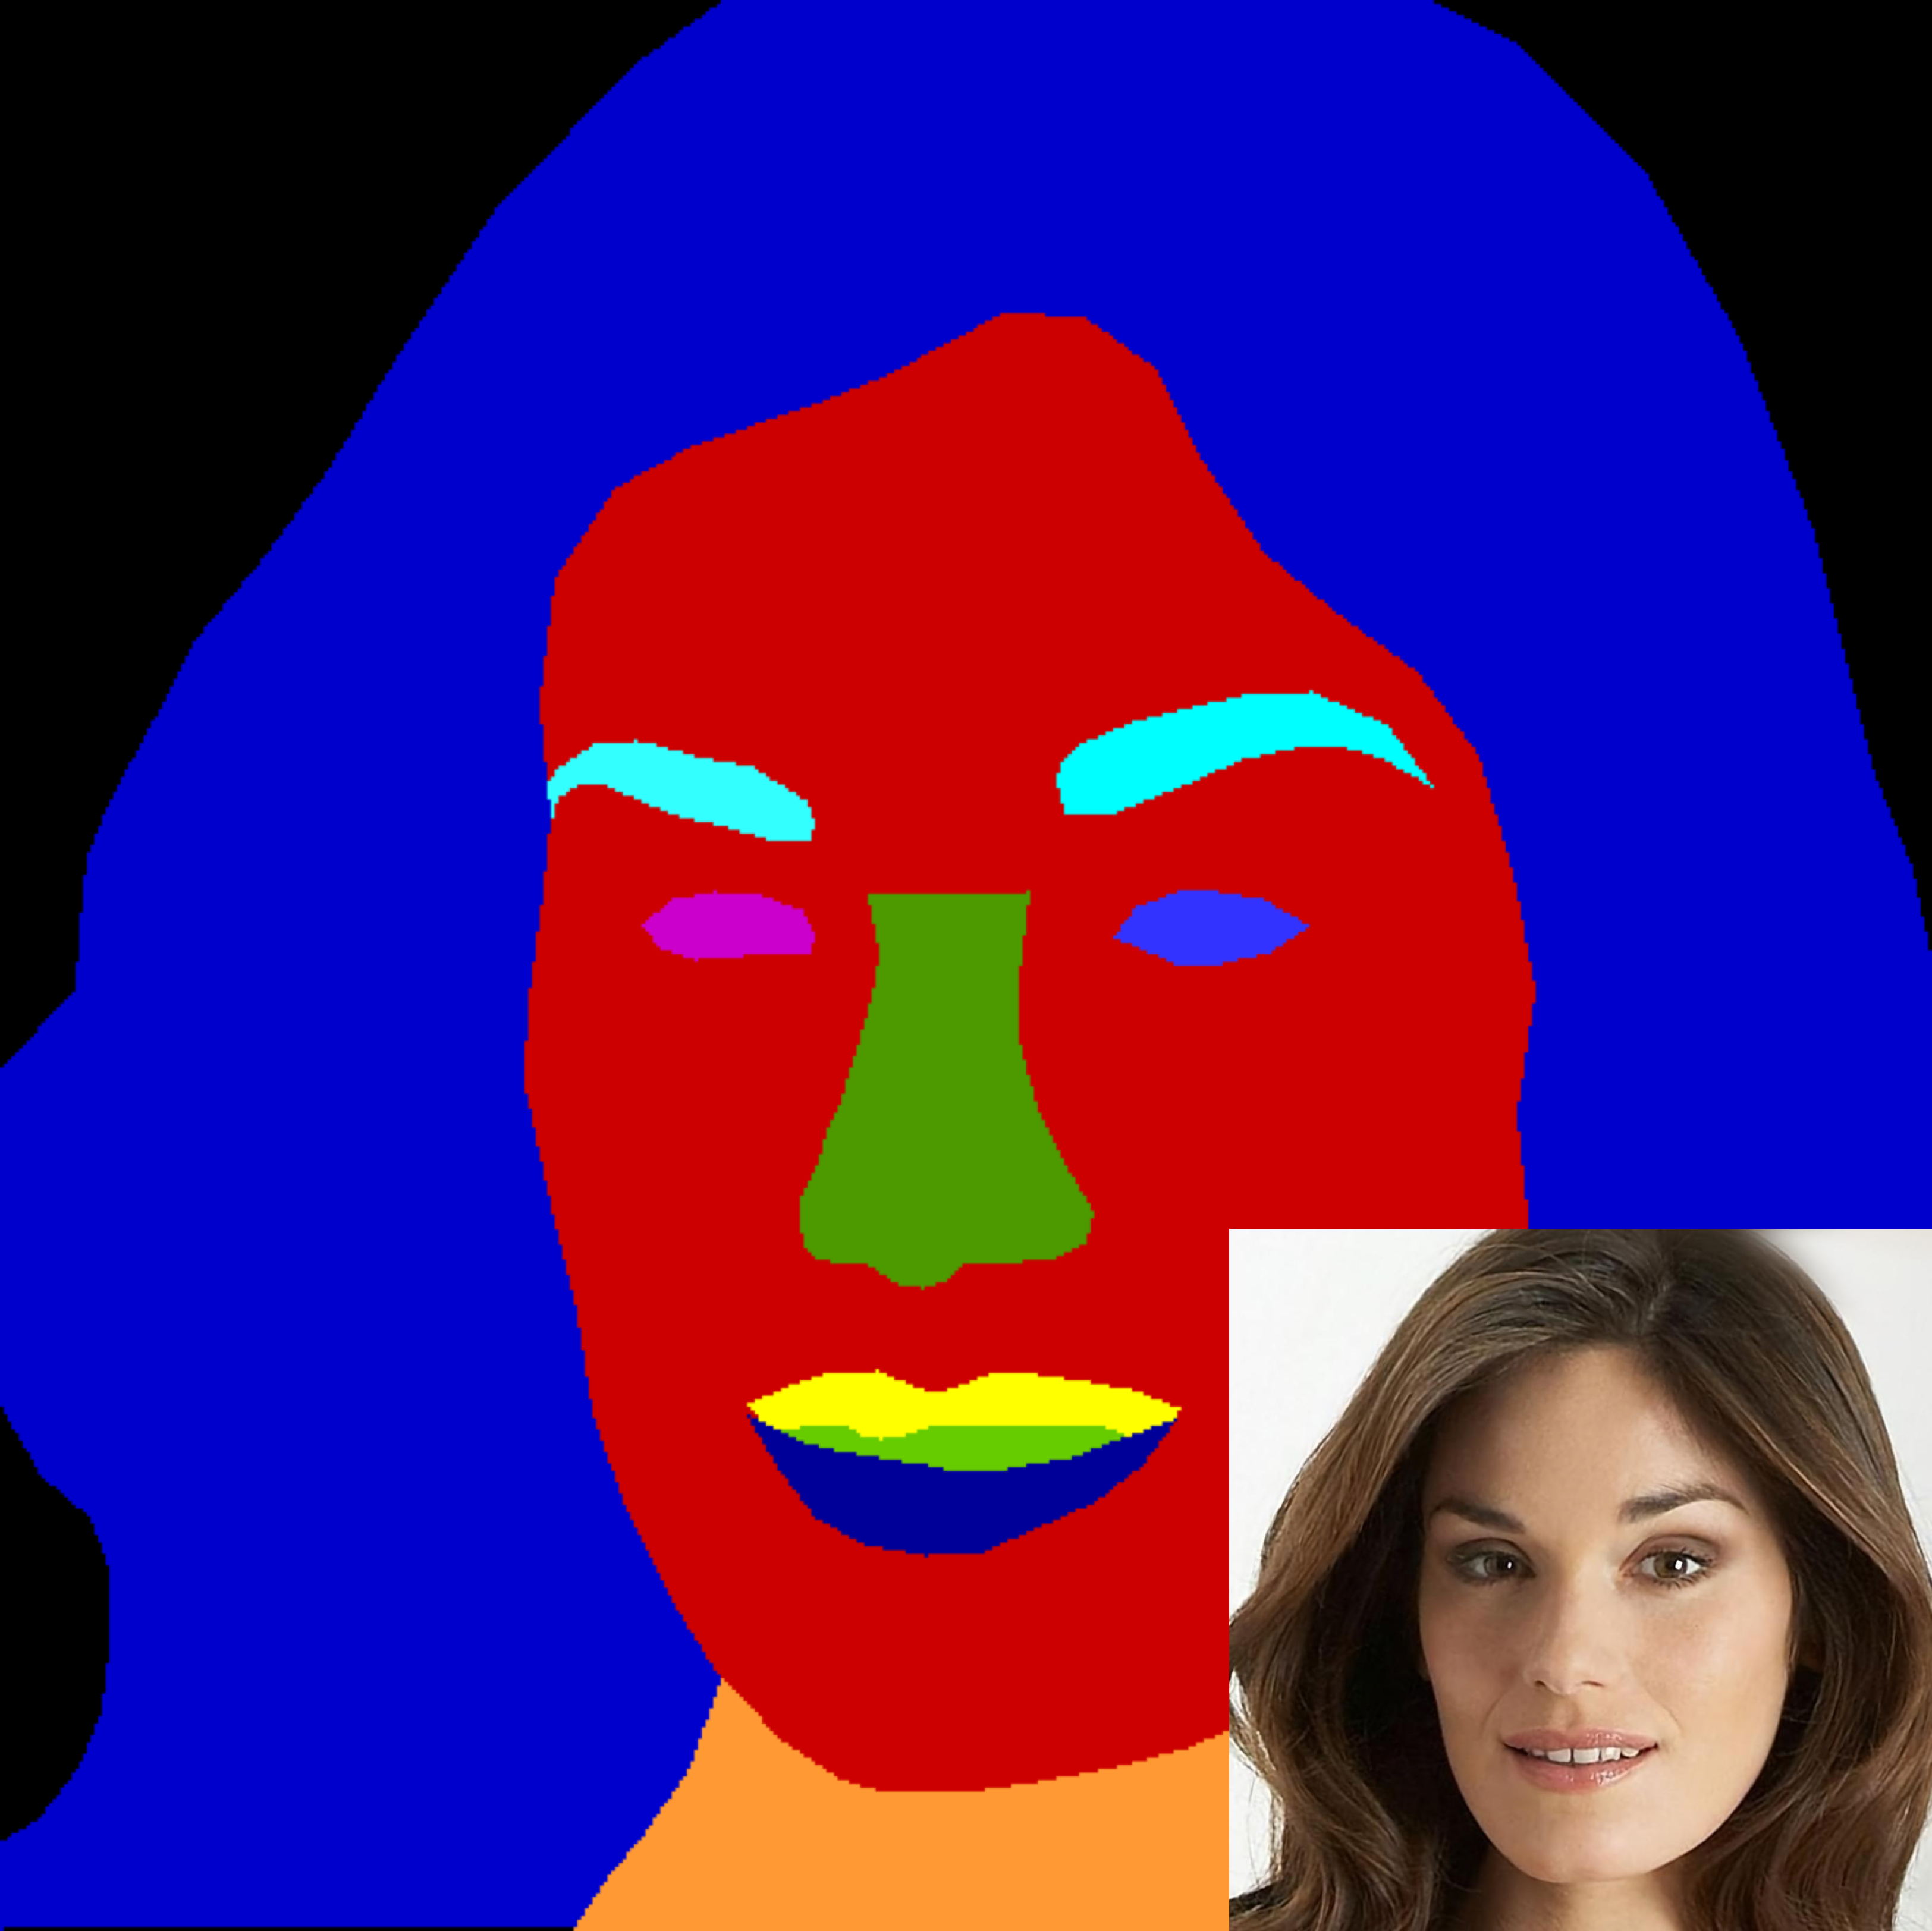
\includegraphics[width=0.11\textwidth]{Images/Encoder_search/encoder_2.png} & 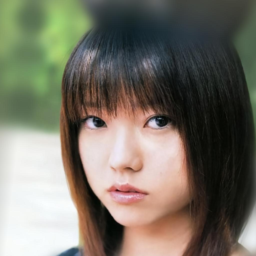
\includegraphics[width=0.11\textwidth]{Images/Encoder_search/style/29573.png} &
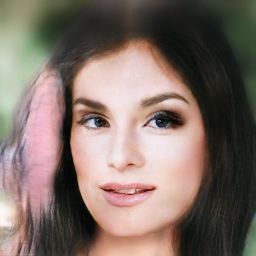
\includegraphics[width=0.11\textwidth]{Images/Encoder_search/SEAN_level/3.png} &   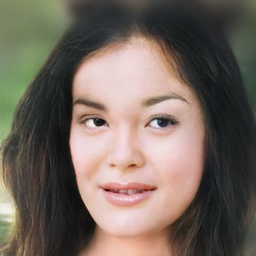
\includegraphics[width=0.11\textwidth]{Images/Encoder_search/Unified/3.png}\\ 

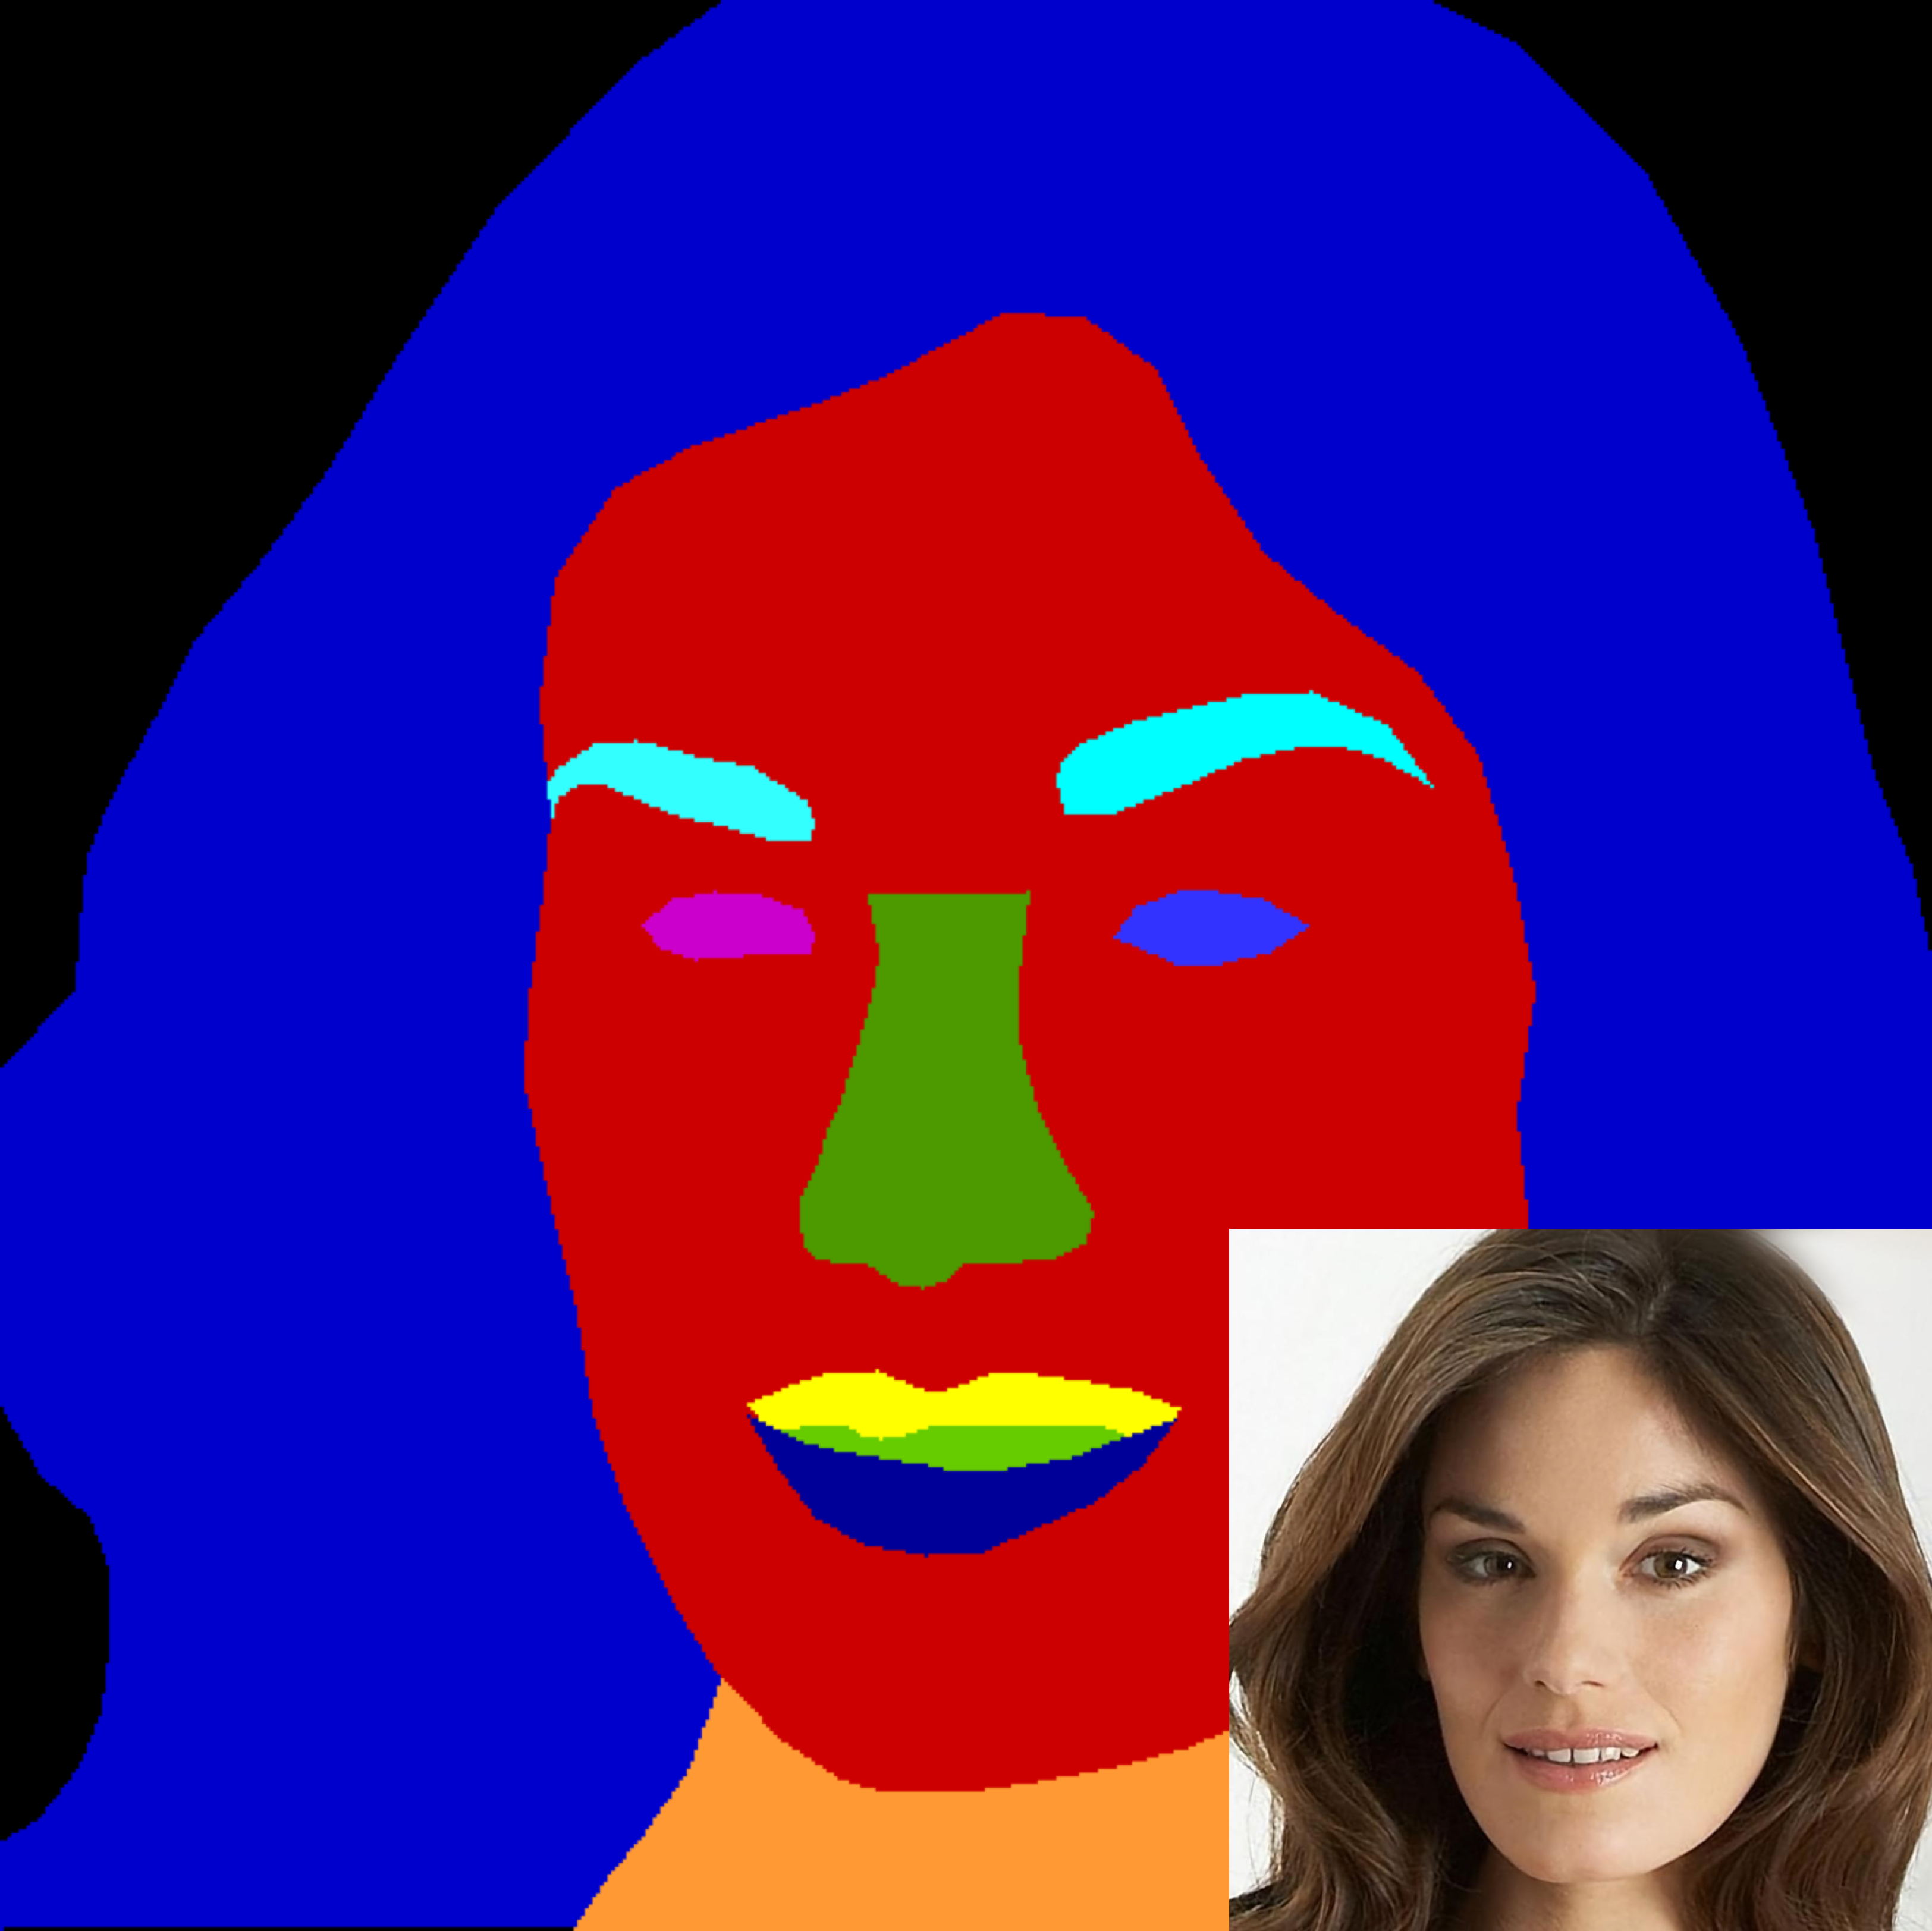
\includegraphics[width=0.11\textwidth]{Images/Encoder_search/encoder_2.png} & 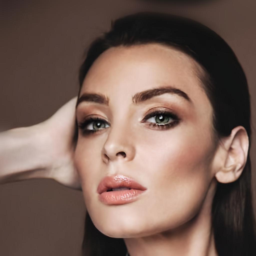
\includegraphics[width=0.11\textwidth]{Images/Encoder_search/style/29659.png} &
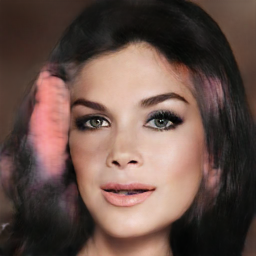
\includegraphics[width=0.11\textwidth]{Images/Encoder_search/SEAN_level/4.png} &   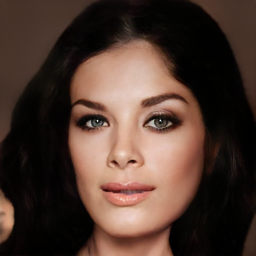
\includegraphics[width=0.11\textwidth]{Images/Encoder_search/Unified/4.png}\\ 


\end{tabular}
\vspace{-2mm}
	\caption{Encoder choice justification. Encoder1 is the SEAN-level encoder and Encoder2 is the unified encoder. SEAN-level encoder is more sensitive to the poses and unlabeled parts of the style image due to the overfitting. Using unified encoder can get more robust style transfer results.}
	\label{fig:Encoder Comparison}	
\vspace{-3mm}	
 \end{figure}
 \egroup
 \addtolength{\tabcolsep}{4.5pt}
%-------------------------------------------------------------------------

\section{Additional Analysis}
\noindent {\bf ST-branch \vs Mask-branch.}
% \noindent {\bf What is the contribution of the two branches to the final result?}
The contributions of ST-branch and mask-branch are determined by a linear combination (parameters $\alpha_\beta$ and $\alpha_\gamma$). The resulting parameters are typically in the range of $0.35 - 0.7$ meaning that both branches are actively contributing to the result. See Fig~\ref{fig:weight histogram} for one example.
It is possible to completely drop the mask-branch, but the results will get worse. 
It was our initial intuition that the mask branch provides the rough structure and the ST-branch additional details. However, in the end, the interaction is quite complicated and cannot be understood by just varying the mixing parameter.


% \vspace*{2mm}

\begin{figure}[h]
\centering
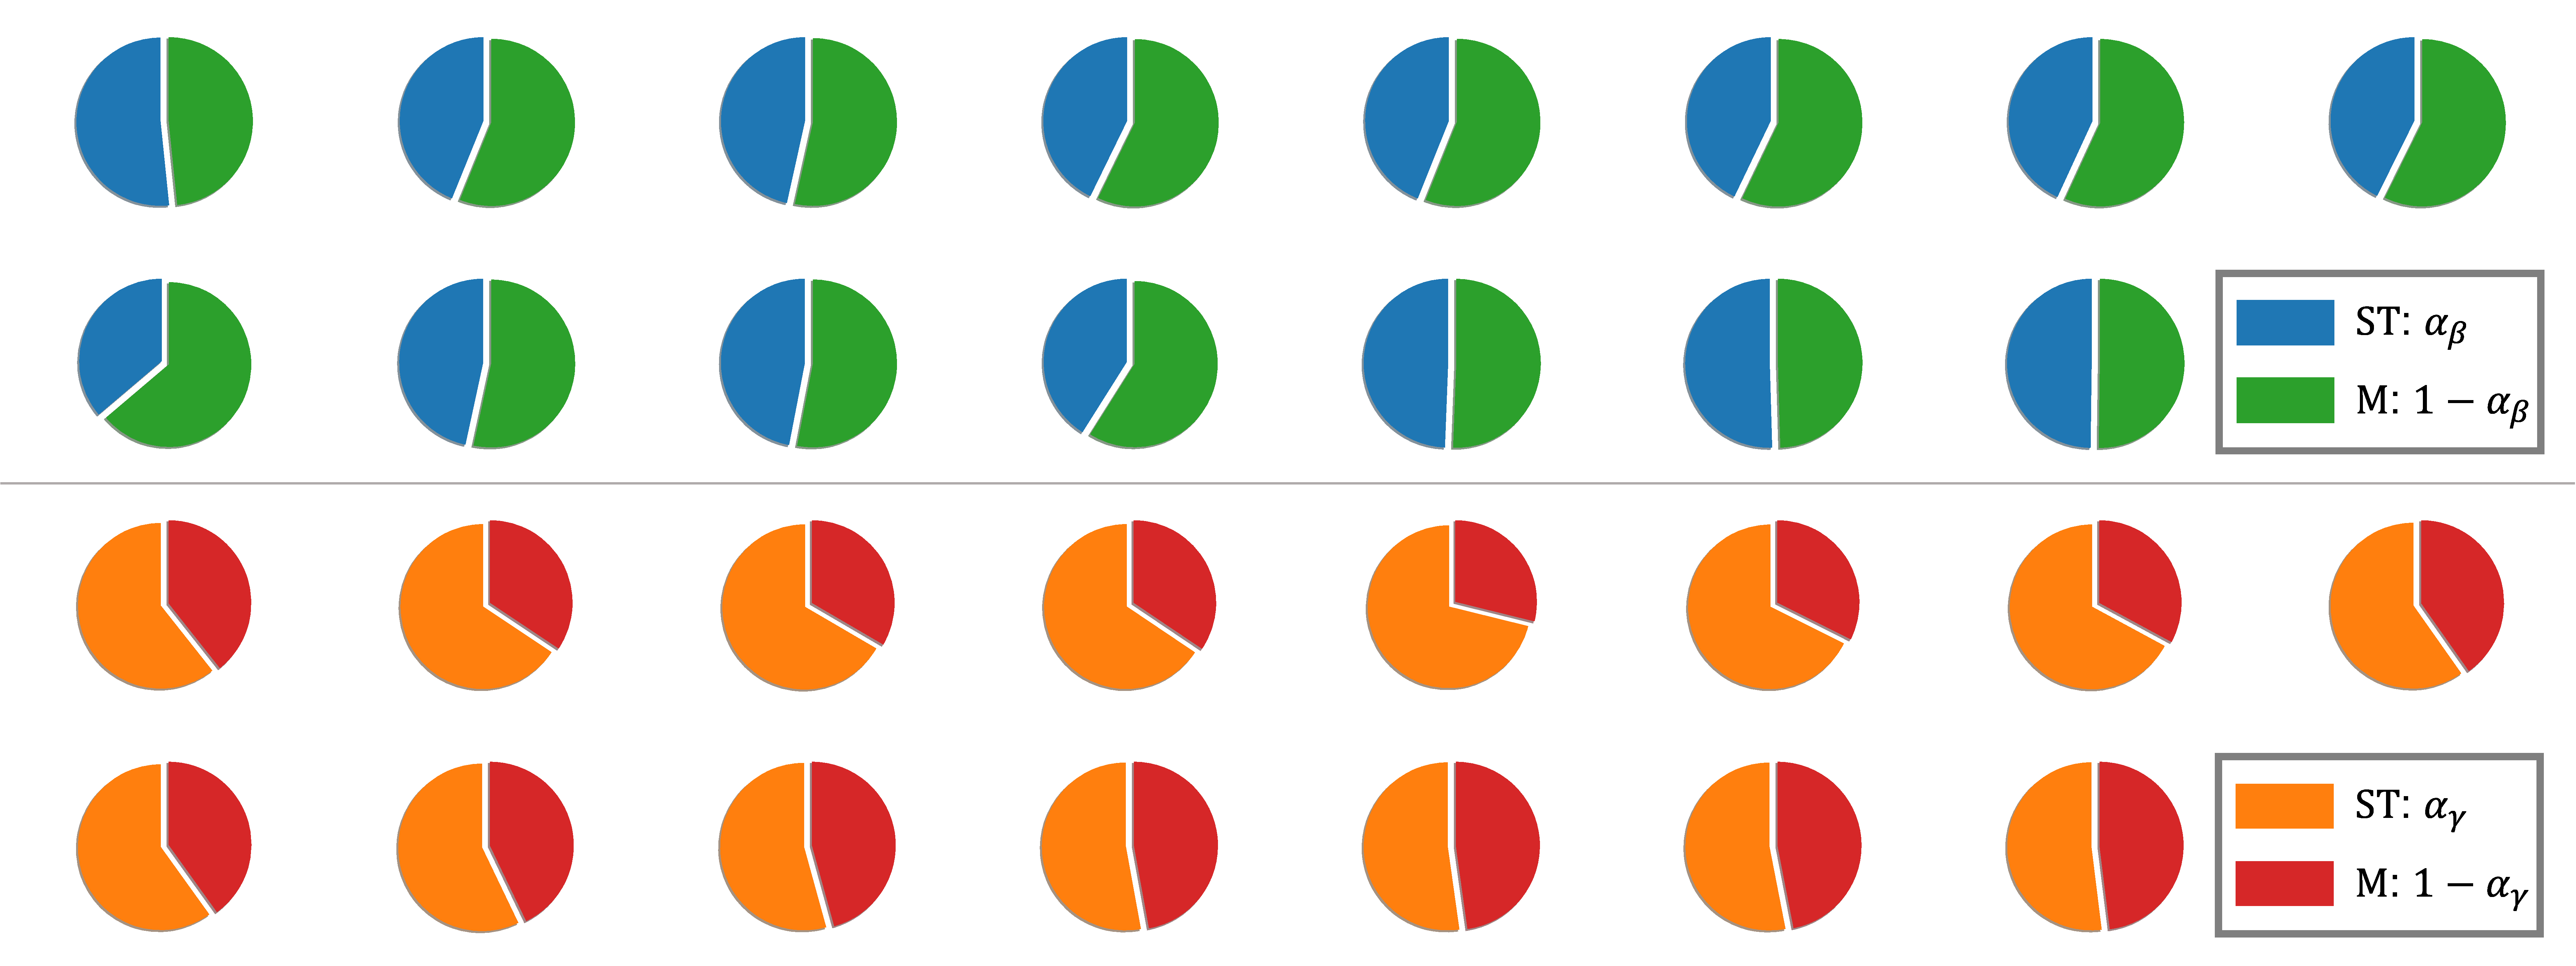
\includegraphics[width=\linewidth]{Rebuttal/histogram.pdf}
\caption{Contributions of ST-branch and Mask-branch for each SEAN normalization block. The pie charts and SEAN normalization blocks are in one-to-one correspondence.}
\label{fig:weight histogram}
\end{figure}


\noindent \textbf{Extreme Cases.}
To further demonstrate SEAN's power in texture transfer, we show that highly complex textures from an artistic image can be transferred to a human face (Fig~\ref{fig:tree}).
\begin{figure}[h]
\centering
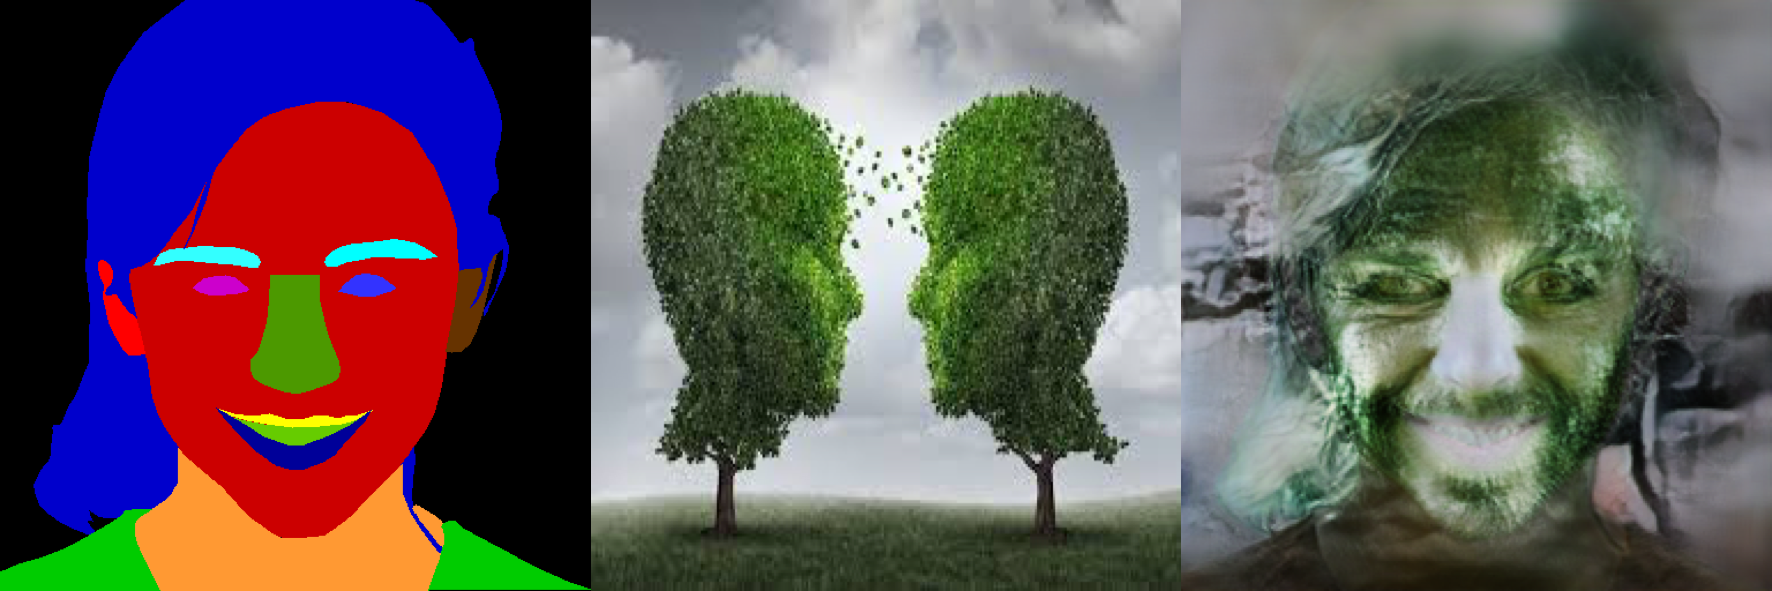
\includegraphics[width=0.8\linewidth]{Rebuttal/tree.png}
\caption{Complex texture transfer.}
\label{fig:tree}
\end{figure}
% \noindent \textbf{What happens if you paint a semantic region at a location where spatially it does not make sense?} 

\vspace*{-5mm}
\noindent In addition, our method is highly flexible that enables users to paint a semantic region at a spatially unreasonable location arbitrarily (Fig~\ref{fig:monster}).
% shows an example that our method allows users to put eyes anywhere on a face.

\begin{figure}[h]
\centering
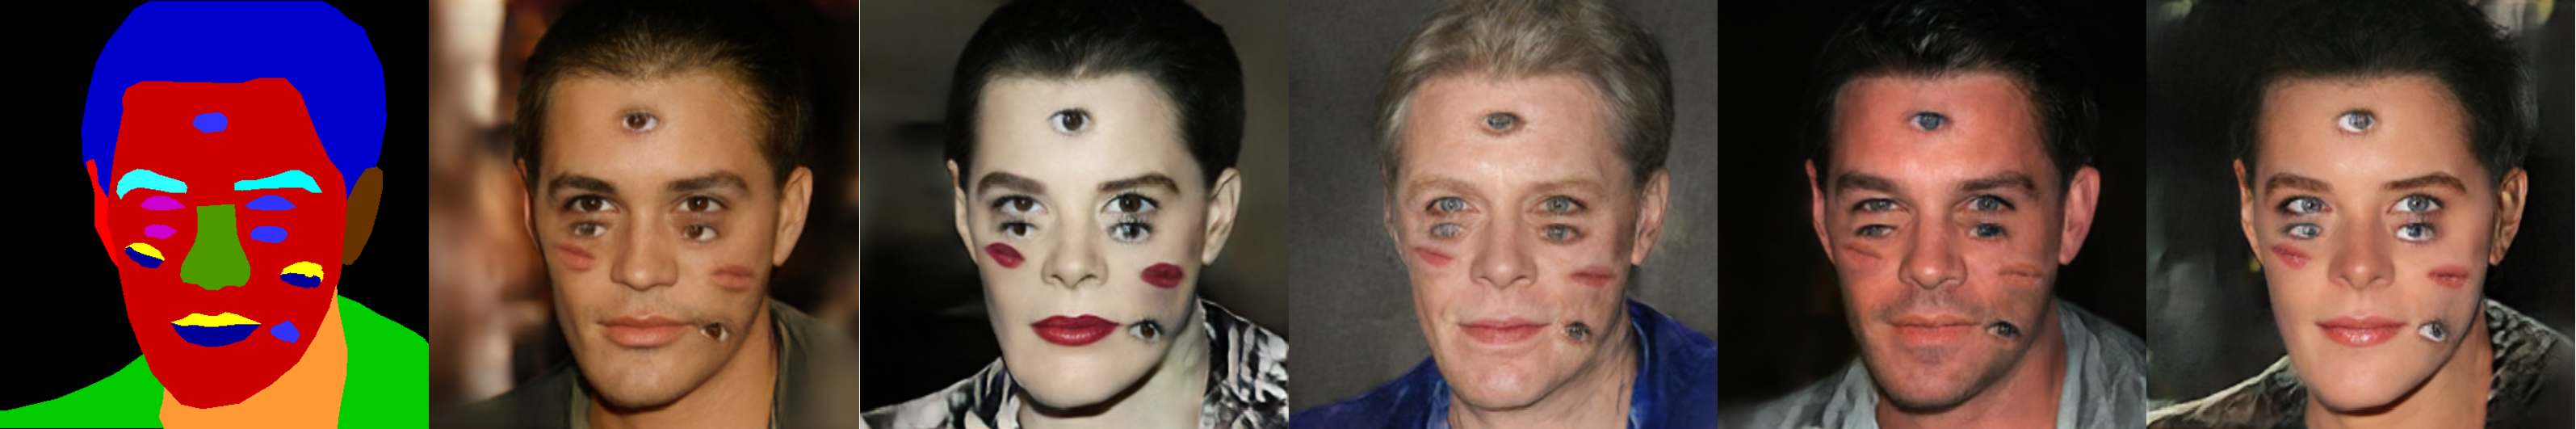
\includegraphics[width=1.0\linewidth]{Rebuttal/monster.pdf}
\caption{Spatially-flexible painting. Our method allows users to put eyes anywhere on a face.}
\label{fig:monster}
\end{figure}



\section{Additional Results}

To demonstrate that the proposed per-region style control method builds the foundation of a highly flexible image-editing software, we designed an interactive UI for a demo.
Our UI enables high quality image synthesis by transferring the per-region styles from various images to an arbitrary segmentation mask.
New styles can be created by interpolating existing styles.
Please find the recorded videos of our demo in the supplementary material.


Figure~\ref{fig:additional style transfer} shows additional style transfer results on CelebAMask-HQ~\cite{CelebAMask-HQ,karras2017progressive,liu2015faceattributes} dataset. Figure~\ref{fig:Supp face interpolation} and Figure~\ref{fig:Supp ADE interpolation} show additional style interpolation results on CelebAMask-HQ and ADE20K datasets.

Figure~\ref{fig:CelebAMask-HQ results}, ~\ref{fig:ADE20K results}, ~\ref{fig:ADE20K outdoor results} and ~\ref{fig:City Facades results} show additional image reconstruction results of our method, Pix2PixHD and SPADE on the CelebAMask-HQ~\cite{CelebAMask-HQ,karras2017progressive,liu2015faceattributes}, ADE20K~\cite{zhou2017scene}, CityScapes~\cite{Cordts2016Cityscapes} and our \Facades datasets respectively.
It can be observed that our reconstructions are of much higher quality than those of Pix2PixHD and SPADE.

\begin{figure*}[th]
\centering
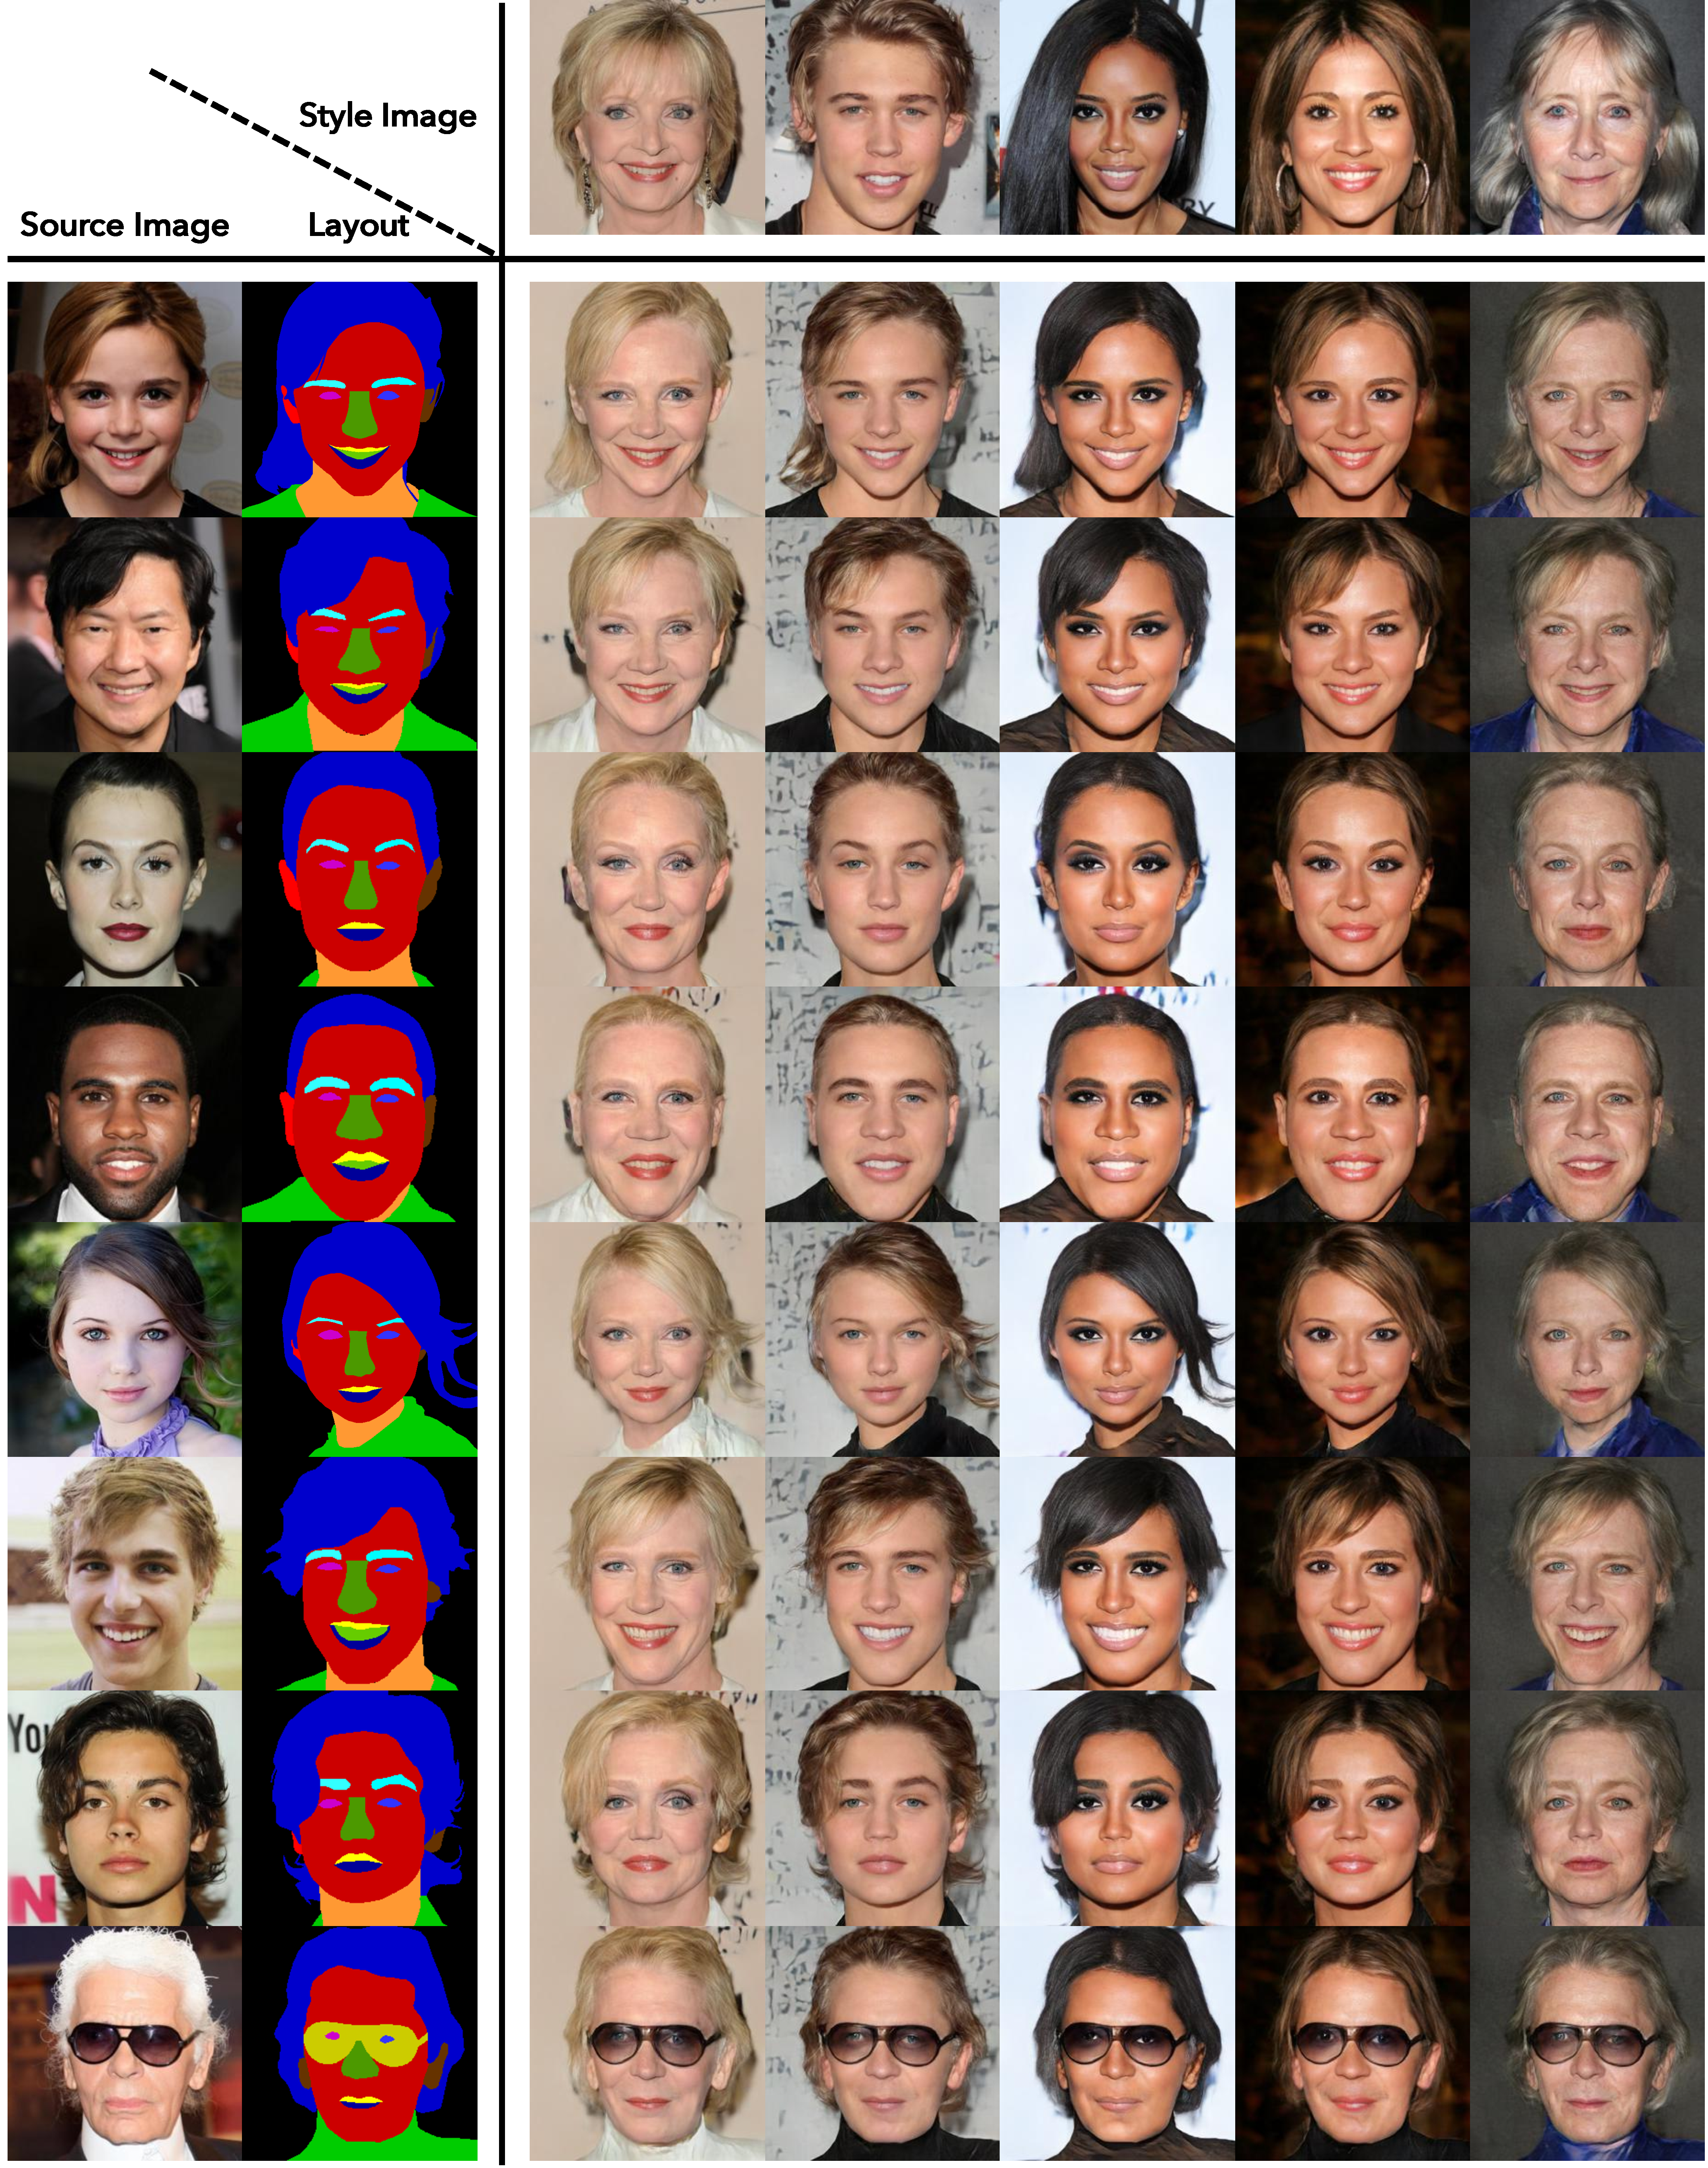
\includegraphics[width=\linewidth]{Figures/Teaser_jpg.pdf}
\caption{Style transfer on CelebAMask-HQ dataset}
\label{fig:additional style transfer}
\end{figure*}


\begin{figure*}[th]
\centering
\includegraphics[width=\linewidth]{Figures/supp_face_interpolation.pdf}
\caption{Style interpolation on CelebAMask-HQ dataset}
\label{fig:Supp face interpolation}
\end{figure*}

\begin{figure*}[th]
\centering
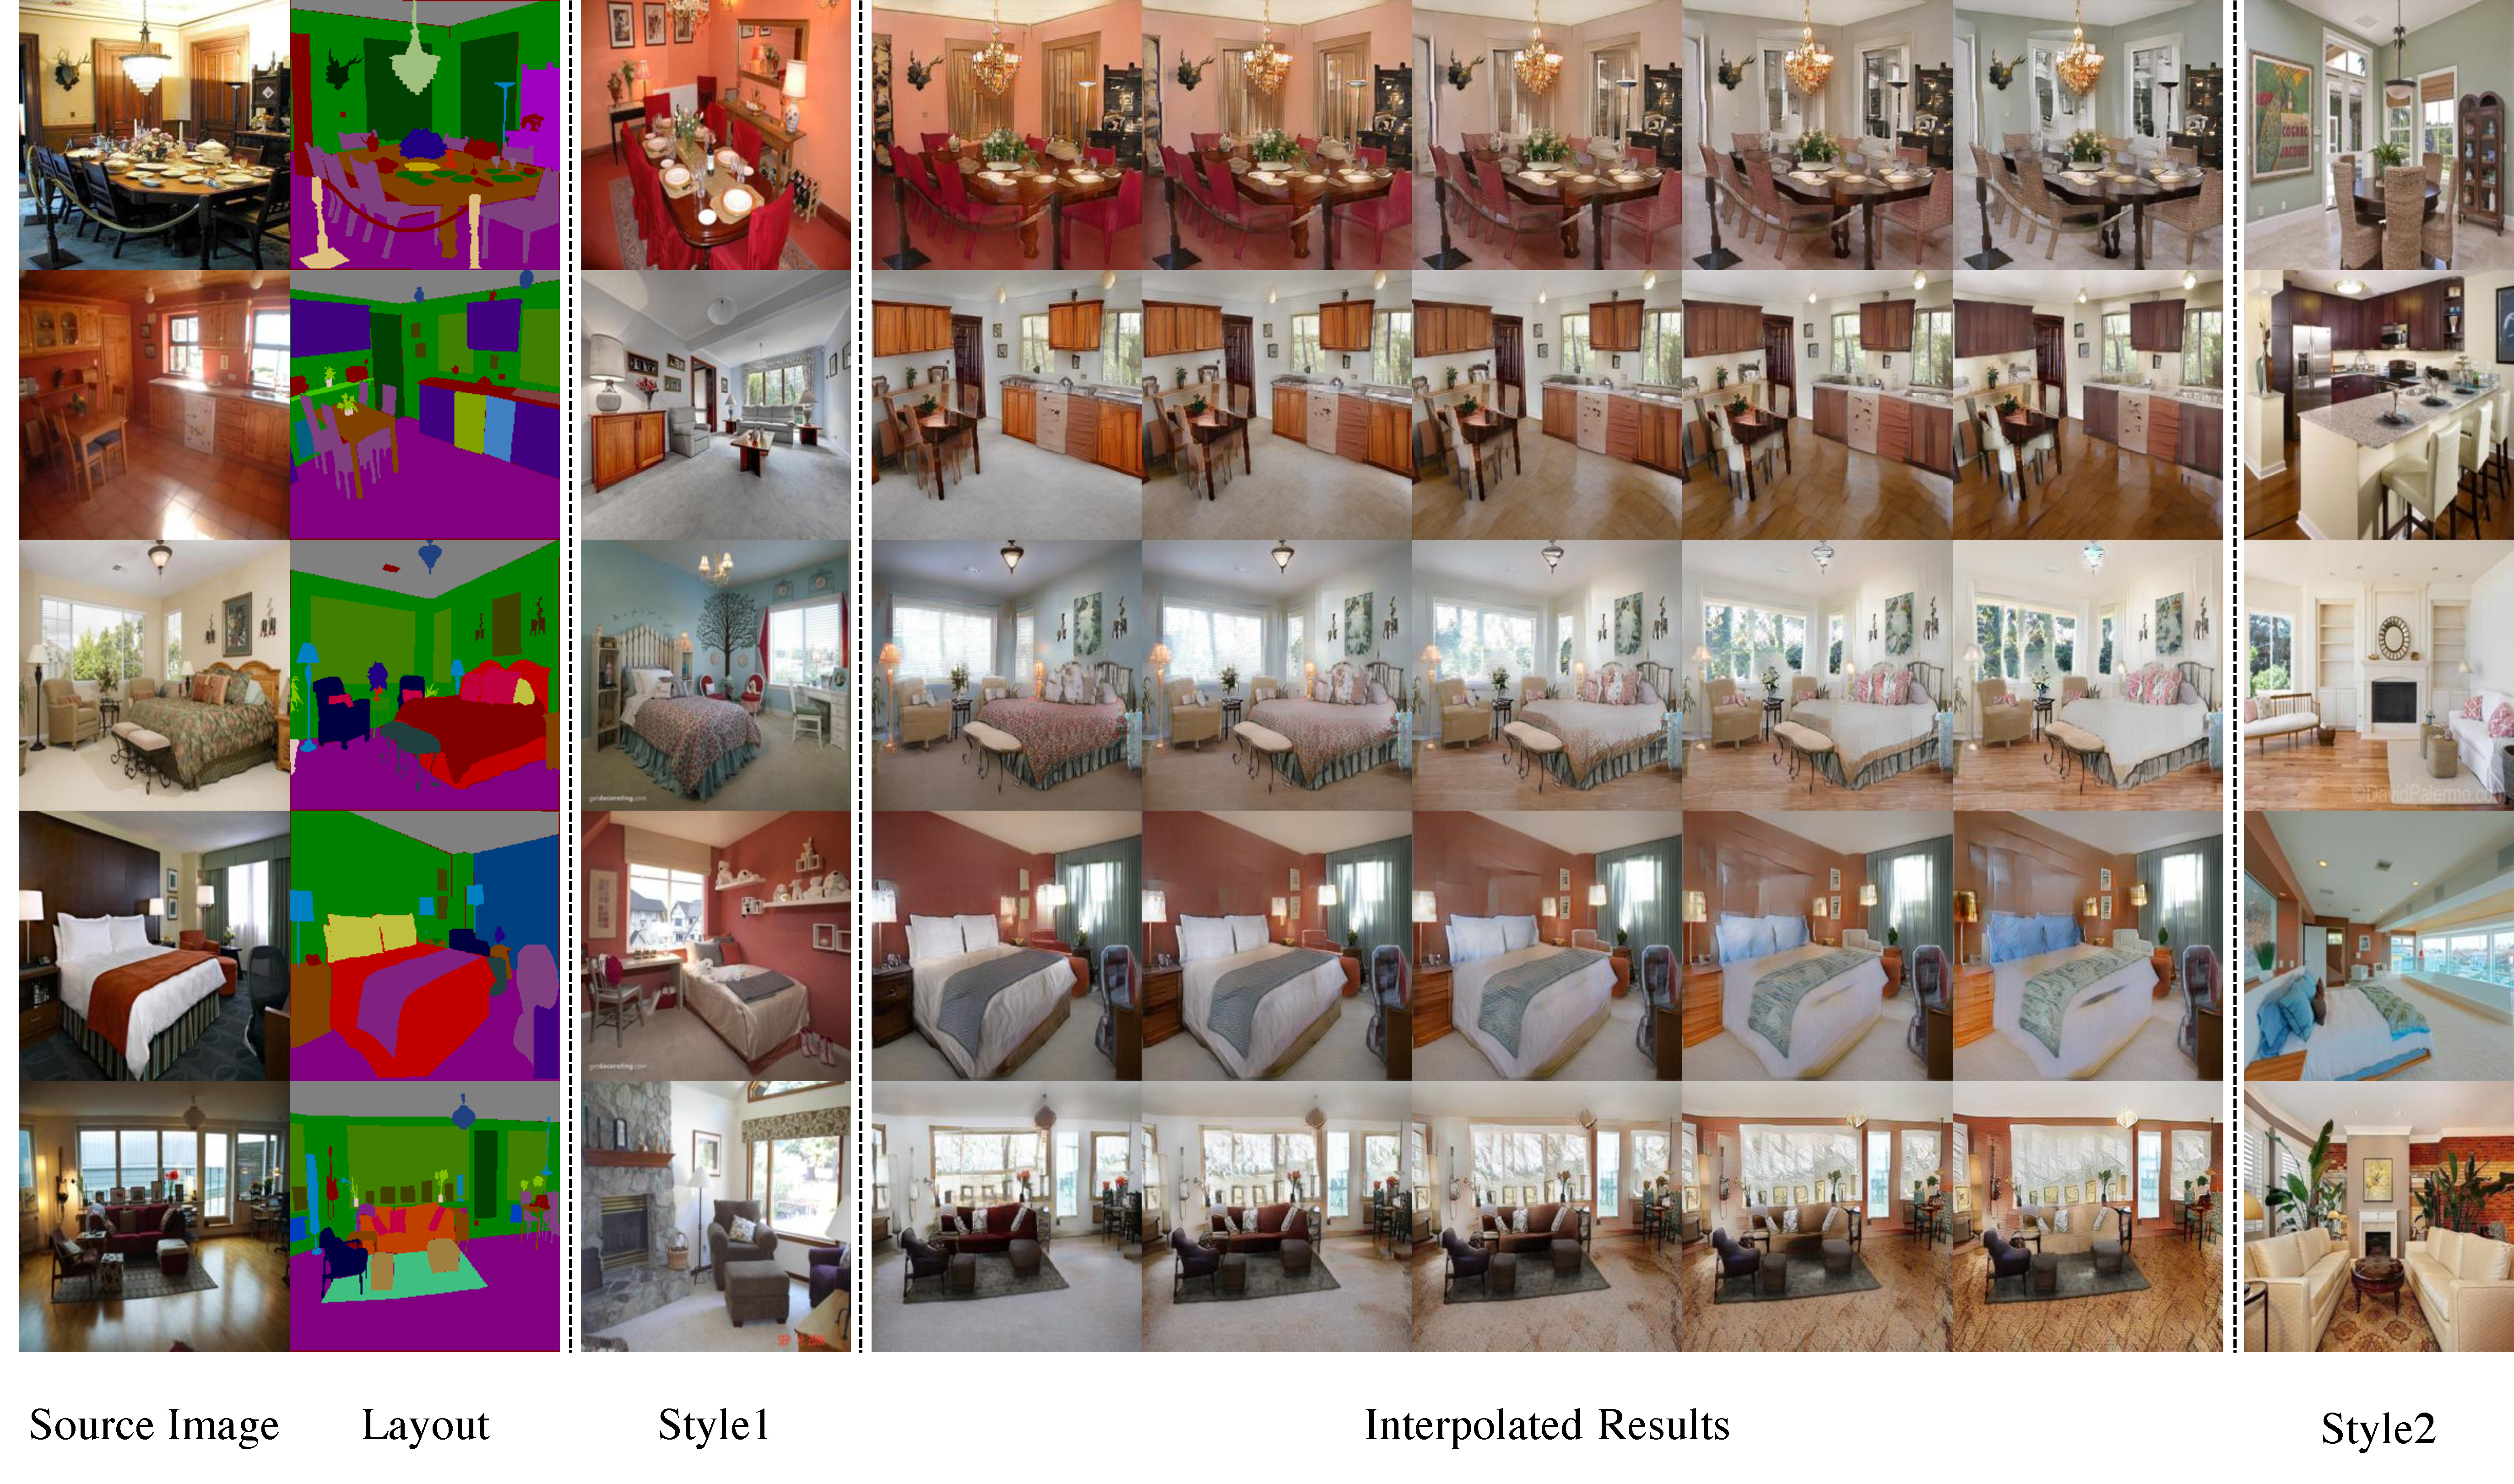
\includegraphics[width=\linewidth]{Figures/supp_ADE_interpolation_jpg.pdf}
\caption{Style interpolation on ADE20K dataset}
\label{fig:Supp ADE interpolation}
\end{figure*}

\addtolength{\tabcolsep}{-4.5pt}    
% \setlength{\mywidth}{0.1932\textwidth}
\bgroup
\def\arraystretch{0.5}%  1 is the default. Controls vertical spacing.
\begin{figure*}[]
\begin{tabular} {cc|cc|c}
 Label & Ground Truth & Pix2PixHD~\cite{wang2018pix2pixHD} &  SPADE~\cite{park2019SPADE} & Ours\\
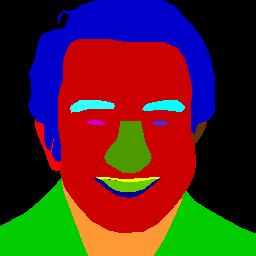
\includegraphics[width=0.1932\textwidth]{Images/Rec/Faces/label/28016.png} & 
\includegraphics[width=0.1932\textwidth]{Images/Rec/Faces/gt/28016.jpg} &
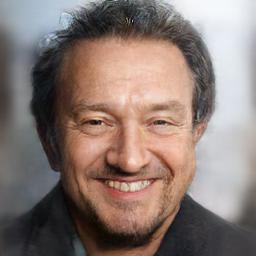
\includegraphics[width=0.1932\textwidth]{Images/Rec/Faces/pix2pixhd/28016.jpg} &   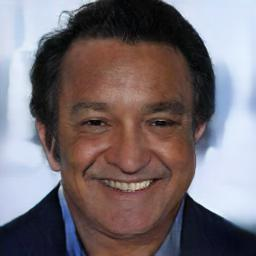
\includegraphics[width=0.1932\textwidth]{Images/Rec/Faces/spade/28016.jpg} &  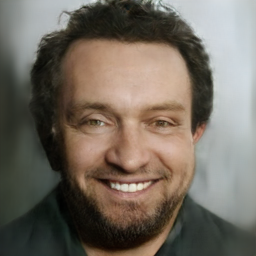
\includegraphics[width=0.1932\textwidth]{Images/Rec/Faces/ours/28016.png} \\



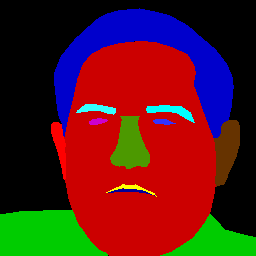
\includegraphics[width=0.1932\textwidth]{Images/Rec/Faces/label/28054.png} & 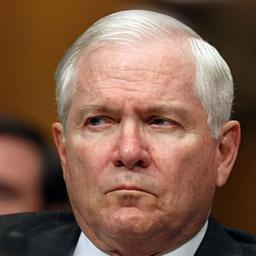
\includegraphics[width=0.1932\textwidth]{Images/Rec/Faces/gt/28054.jpg} &
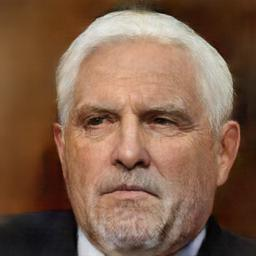
\includegraphics[width=0.1932\textwidth]{Images/Rec/Faces/pix2pixhd/28054.jpg}&
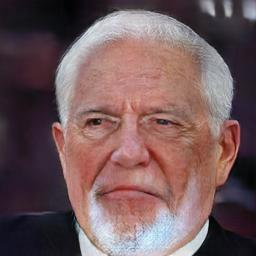
\includegraphics[width=0.1932\textwidth]{Images/Rec/Faces/spade/28054.jpg} &  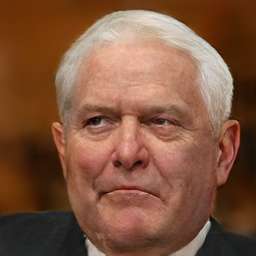
\includegraphics[width=0.1932\textwidth]{Images/Rec/Faces/ours/28054.png} \\



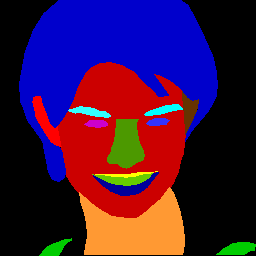
\includegraphics[width=0.1932\textwidth]{Images/Rec/Faces/label/28434.png} & 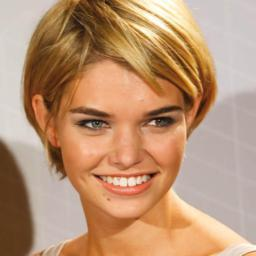
\includegraphics[width=0.1932\textwidth]{Images/Rec/Faces/gt/28434.jpg} &
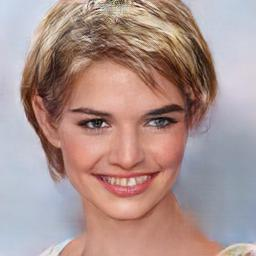
\includegraphics[width=0.1932\textwidth]{Images/Rec/Faces/pix2pixhd/28434.jpg}&
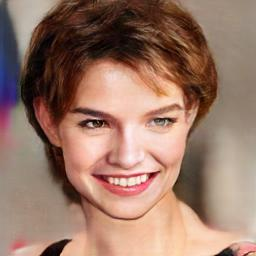
\includegraphics[width=0.1932\textwidth]{Images/Rec/Faces/spade/28434.jpg} &  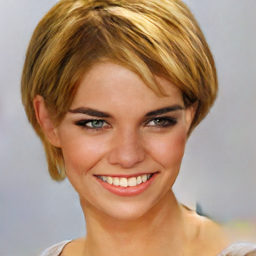
\includegraphics[width=0.1932\textwidth]{Images/Rec/Faces/ours/28434.png} \\

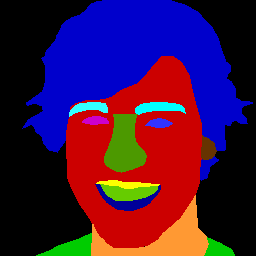
\includegraphics[width=0.1932\textwidth]{Images/Rec/Faces/label/28092.png} & 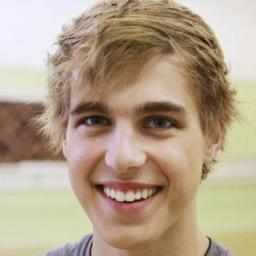
\includegraphics[width=0.1932\textwidth]{Images/Rec/Faces/gt/28092.jpg} &
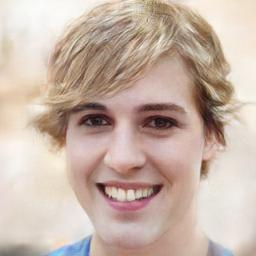
\includegraphics[width=0.1932\textwidth]{Images/Rec/Faces/pix2pixhd/28092.jpg} &   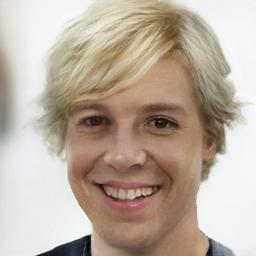
\includegraphics[width=0.1932\textwidth]{Images/Rec/Faces/spade/28092.jpg} &  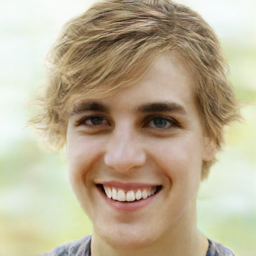
\includegraphics[width=0.1932\textwidth]{Images/Rec/Faces/ours/28092.png} \\

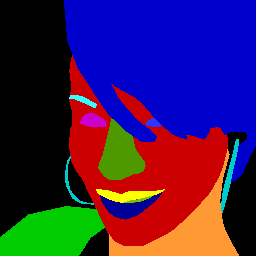
\includegraphics[width=0.1932\textwidth]{Images/Rec/Faces/label/28053.png} & 
\includegraphics[width=0.1932\textwidth]{Images/Rec/Faces/gt/28053.jpg} &

\includegraphics[width=0.1932\textwidth]{Images/Rec/Faces/pix2pixhd/28053.jpg} &   
\includegraphics[width=0.1932\textwidth]{Images/Rec/Faces/spade/28053.jpg} &  \includegraphics[width=0.1932\textwidth]{Images/Rec/Faces/ours/28053.png} \\

\includegraphics[width=0.1932\textwidth]{Images/Rec/Faces/label/28059.png} & \includegraphics[width=0.1932\textwidth]{Images/Rec/Faces/gt/28059.jpg} &
\includegraphics[width=0.1932\textwidth]{Images/Rec/Faces/pix2pixhd/28059.jpg} &   \includegraphics[width=0.1932\textwidth]{Images/Rec/Faces/spade/28059.jpg} &  \includegraphics[width=0.1932\textwidth]{Images/Rec/Faces/ours/28059.png} \\





\end{tabular}
\vspace{-2mm}
	\caption{Visual  comparison  of  semantic  image  synthesis  results  on  the  CelebAMask-HQ dataset. We compare Pix2PixHD, SPADE, and our method.}
	\label{fig:CelebAMask-HQ results}	
\vspace{-3mm}	
 \end{figure*}
 \egroup
 \addtolength{\tabcolsep}{4.5pt}

\addtolength{\tabcolsep}{-4.5pt}    
% \setlength{\mywidth}{0.1932\textwidth}
\bgroup
\def\arraystretch{0.5}%  1 is the default. Controls vertical spacing.
\begin{figure*}[]
\begin{tabular} {cc|cc|c}
 Label & Ground Truth & Pix2PixHD~\cite{wang2018pix2pixHD} &  SPADE~\cite{park2019SPADE} & Ours\\


\includegraphics[width=0.1932\textwidth,height=0.96in]{Images/Rec/ADE/label/ADE_val_00000244.png} & \includegraphics[width=0.1932\textwidth,height=0.96in]{Images/Rec/ADE/gt/ADE_val_00000244.jpg} &
\includegraphics[width=0.1932\textwidth,height=0.96in]{Images/Rec/ADE/pix2pixhd/ADE_val_00000244.jpg} &   \includegraphics[width=0.1932\textwidth,height=0.96in]{Images/Rec/ADE/spade/ADE_val_00000244.jpg} &  \includegraphics[width=0.1932\textwidth,height=0.96in]{Images/Rec/ADE/ours/ADE_val_00000244.png} \\


\includegraphics[width=0.1932\textwidth,height=0.96in]{Images/Rec/ADE/label/ADE_val_00000309.png} & \includegraphics[width=0.1932\textwidth,height=0.96in]{Images/Rec/ADE/gt/ADE_val_00000309.jpg} &
\includegraphics[width=0.1932\textwidth,height=0.96in]{Images/Rec/ADE/pix2pixhd/ADE_val_00000309.jpg} &   \includegraphics[width=0.1932\textwidth,height=0.96in]{Images/Rec/ADE/spade/ADE_val_00000309.jpg} &  \includegraphics[width=0.1932\textwidth,height=0.96in]{Images/Rec/ADE/ours/ADE_val_00000309.png} \\


\includegraphics[width=0.1932\textwidth,height=0.96in]{Images/Rec/ADE/label/ADE_val_00001090.png} & \includegraphics[width=0.1932\textwidth,height=0.96in]{Images/Rec/ADE/gt/ADE_val_00001090.jpg} &
\includegraphics[width=0.1932\textwidth,height=0.96in]{Images/Rec/ADE/pix2pixhd/ADE_val_00001090.jpg} &   \includegraphics[width=0.1932\textwidth,height=0.96in]{Images/Rec/ADE/spade/ADE_val_00001090.jpg} &  \includegraphics[width=0.1932\textwidth,height=0.96in]{Images/Rec/ADE/ours/ADE_val_00001090.png} \\

\includegraphics[width=0.1932\textwidth,height=0.96in]{Images/Rec/ADE/label/ADE_val_00001243.png} & \includegraphics[width=0.1932\textwidth,height=0.96in]{Images/Rec/ADE/gt/ADE_val_00001243.jpg} &
\includegraphics[width=0.1932\textwidth,height=0.96in]{Images/Rec/ADE/pix2pixhd/ADE_val_00001243.jpg} &   \includegraphics[width=0.1932\textwidth,height=0.96in]{Images/Rec/ADE/spade/ADE_val_00001243.jpg} &  \includegraphics[width=0.1932\textwidth,height=0.96in]{Images/Rec/ADE/ours/ADE_val_00001243.png} \\


\includegraphics[width=0.1932\textwidth,height=0.96in]{Images/Rec/ADE/label/ADE_val_00001517.png} & \includegraphics[width=0.1932\textwidth,height=0.96in]{Images/Rec/ADE/gt/ADE_val_00001517.jpg} &
\includegraphics[width=0.1932\textwidth,height=0.96in]{Images/Rec/ADE/pix2pixhd/ADE_val_00001517.jpg} &   \includegraphics[width=0.1932\textwidth,height=0.96in]{Images/Rec/ADE/spade/ADE_val_00001517.jpg} &  \includegraphics[width=0.1932\textwidth,height=0.96in]{Images/Rec/ADE/ours/ADE_val_00001517.png} \\

\includegraphics[width=0.1932\textwidth,height=0.96in]{Images/Rec/ADE/label/ADE_val_00000090.png} & \includegraphics[width=0.1932\textwidth,height=0.96in]{Images/Rec/ADE/gt/ADE_val_00000090.jpg} &
\includegraphics[width=0.1932\textwidth,height=0.96in]{Images/Rec/ADE/pix2pixhd/ADE_val_00000090.jpg} &   \includegraphics[width=0.1932\textwidth,height=0.96in]{Images/Rec/ADE/spade/ADE_val_00000090.jpg} &  \includegraphics[width=0.1932\textwidth,height=0.96in]{Images/Rec/ADE/ours/ADE_val_00000090.png} \\

\includegraphics[width=0.1932\textwidth,height=0.96in]{Images/Rec/ADE/label/ADE_val_00000107.png} & \includegraphics[width=0.1932\textwidth,height=0.96in]{Images/Rec/ADE/gt/ADE_val_00000107.jpg} &
\includegraphics[width=0.1932\textwidth,height=0.96in]{Images/Rec/ADE/pix2pixhd/ADE_val_00000107.jpg} &   \includegraphics[width=0.1932\textwidth,height=0.96in]{Images/Rec/ADE/spade/ADE_val_00000107.jpg} &  \includegraphics[width=0.1932\textwidth,height=0.96in]{Images/Rec/ADE/ours/ADE_val_00000107.png} \\

% \includegraphics[width=0.1932\textwidth,height=0.96in]{Images/Rec/ADE/label/ADE_val_00000163.png} & \includegraphics[width=0.1932\textwidth,height=0.96in]{Images/Rec/ADE/gt/ADE_val_00000163.png} &
% \includegraphics[width=0.1932\textwidth,height=0.96in]{Images/Rec/ADE/pix2pixhd/ADE_val_00000163.png} &   \includegraphics[width=0.1932\textwidth,height=0.96in]{Images/Rec/ADE/spade/ADE_val_00000163.png} &  \includegraphics[width=0.1932\textwidth,height=0.96in]{Images/Rec/ADE/ours/ADE_val_00000163.png} \\

\includegraphics[width=0.1932\textwidth,height=0.96in]{Images/Rec/ADE/label/ADE_val_00000969.png} & \includegraphics[width=0.1932\textwidth,height=0.96in]{Images/Rec/ADE/gt/ADE_val_00000969.jpg} &
\includegraphics[width=0.1932\textwidth,height=0.96in]{Images/Rec/ADE/pix2pixhd/ADE_val_00000969.jpg} &   \includegraphics[width=0.1932\textwidth,height=0.96in]{Images/Rec/ADE/spade/ADE_val_00000969.jpg} &  \includegraphics[width=0.1932\textwidth,height=0.96in]{Images/Rec/ADE/ours/ADE_val_00000969.png} \\


\end{tabular}
\vspace{-2mm}
	\caption{Visual  comparison  of  semantic  image  synthesis  results  on  the ADE20K dataset. We compare Pix2PixHD, SPADE, and our method.}
	\label{fig:ADE20K results}	
\vspace{-3mm}	
 \end{figure*}
 \egroup
 \addtolength{\tabcolsep}{4.5pt}

\addtolength{\tabcolsep}{-4.5pt}    
% \setlength{\mywidth}{0.1932\textwidth}
\bgroup
\def\arraystretch{0.5}%  1 is the default. Controls vertical spacing.
\begin{figure*}[]
\begin{tabular} {cc|cc|c}
 Label & Ground Truth & Pix2PixHD~\cite{wang2018pix2pixHD} &  SPADE~\cite{park2019SPADE} & Ours\\

\includegraphics[width=0.1932\textwidth,height=0.96in]{Images/Rec/ADE_outdoor/label/ADE_val_00000291.png} &
\includegraphics[width=0.1932\textwidth,height=0.96in]{Images/Rec/ADE_outdoor/gt/ADE_val_00000291.jpg} & 
\includegraphics[width=0.1932\textwidth,height=0.96in]{Images/Rec/ADE_outdoor/pix2pixhd/ADE_val_00000291.jpg} &   \includegraphics[width=0.1932\textwidth,height=0.96in]{Images/Rec/ADE_outdoor/spade/ADE_val_00000291.jpg} &  \includegraphics[width=0.1932\textwidth,height=0.96in]{Images/Rec/ADE_outdoor/ours/ADE_val_00000291.png} \\

\includegraphics[width=0.1932\textwidth,height=0.96in]{Images/Rec/ADE_outdoor/label/ADE_val_00000343.png} &
\includegraphics[width=0.1932\textwidth,height=0.96in]{Images/Rec/ADE_outdoor/gt/ADE_val_00000343.jpg} & 
\includegraphics[width=0.1932\textwidth,height=0.96in]{Images/Rec/ADE_outdoor/pix2pixhd/ADE_val_00000343.jpg} &   \includegraphics[width=0.1932\textwidth,height=0.96in]{Images/Rec/ADE_outdoor/spade/ADE_val_00000343.jpg} &  \includegraphics[width=0.1932\textwidth,height=0.96in]{Images/Rec/ADE_outdoor/ours/ADE_val_00000343.png} \\

% \includegraphics[width=0.1932\textwidth,height=0.96in]{Images/Rec/ADE_outdoor/label/ADE_val_00000345.png} &
% \includegraphics[width=0.1932\textwidth,height=0.96in]{Images/Rec/ADE_outdoor/gt/ADE_val_00000345.png} & 
% \includegraphics[width=0.1932\textwidth,height=0.96in]{Images/Rec/ADE_outdoor/pix2pixhd/ADE_val_00000345.png} &   \includegraphics[width=0.1932\textwidth,height=0.96in]{Images/Rec/ADE_outdoor/spade/ADE_val_00000345.png} &  \includegraphics[width=0.1932\textwidth,height=0.96in]{Images/Rec/ADE_outdoor/ours/ADE_val_00000345.png} \\

\includegraphics[width=0.1932\textwidth,height=0.96in]{Images/Rec/ADE_outdoor/label/ADE_val_00000541.png} &
\includegraphics[width=0.1932\textwidth,height=0.96in]{Images/Rec/ADE_outdoor/gt/ADE_val_00000541.jpg} & 
\includegraphics[width=0.1932\textwidth,height=0.96in]{Images/Rec/ADE_outdoor/pix2pixhd/ADE_val_00000541.jpg} &   \includegraphics[width=0.1932\textwidth,height=0.96in]{Images/Rec/ADE_outdoor/spade/ADE_val_00000541.jpg} &  \includegraphics[width=0.1932\textwidth,height=0.96in]{Images/Rec/ADE_outdoor/ours/ADE_val_00000541.png} \\

\includegraphics[width=0.1932\textwidth,height=0.96in]{Images/Rec/ADE_outdoor/label/ADE_val_00000556.png} & \includegraphics[width=0.1932\textwidth,height=0.96in]{Images/Rec/ADE_outdoor/gt/ADE_val_00000556.jpg} &
\includegraphics[width=0.1932\textwidth,height=0.96in]{Images/Rec/ADE_outdoor/pix2pixhd/ADE_val_00000556.jpg} &   \includegraphics[width=0.1932\textwidth,height=0.96in]{Images/Rec/ADE_outdoor/spade/ADE_val_00000556.jpg} &  \includegraphics[width=0.1932\textwidth,height=0.96in]{Images/Rec/ADE_outdoor/ours/ADE_val_00000556.png} \\

\includegraphics[width=0.1932\textwidth,height=0.96in]{Images/Rec/ADE_outdoor/label/ADE_val_00000582.png} & \includegraphics[width=0.1932\textwidth,height=0.96in]{Images/Rec/ADE_outdoor/gt/ADE_val_00000582.jpg} &
\includegraphics[width=0.1932\textwidth,height=0.96in]{Images/Rec/ADE_outdoor/pix2pixhd/ADE_val_00000582.jpg} &   \includegraphics[width=0.1932\textwidth,height=0.96in]{Images/Rec/ADE_outdoor/spade/ADE_val_00000582.jpg} &  \includegraphics[width=0.1932\textwidth,height=0.96in]{Images/Rec/ADE_outdoor/ours/ADE_val_00000582.png} \\

\includegraphics[width=0.1932\textwidth,height=0.96in]{Images/Rec/ADE_outdoor/label/ADE_val_00000662.png} & \includegraphics[width=0.1932\textwidth,height=0.96in]{Images/Rec/ADE_outdoor/gt/ADE_val_00000662.jpg} &
\includegraphics[width=0.1932\textwidth,height=0.96in]{Images/Rec/ADE_outdoor/pix2pixhd/ADE_val_00000662.jpg} &   \includegraphics[width=0.1932\textwidth,height=0.96in]{Images/Rec/ADE_outdoor/spade/ADE_val_00000662.jpg} &  \includegraphics[width=0.1932\textwidth,height=0.96in]{Images/Rec/ADE_outdoor/ours/ADE_val_00000662.png} \\

\includegraphics[width=0.1932\textwidth,height=0.96in]{Images/Rec/ADE_outdoor/label/ADE_val_00001597.png} & \includegraphics[width=0.1932\textwidth,height=0.96in]{Images/Rec/ADE_outdoor/gt/ADE_val_00001597.jpg} &
\includegraphics[width=0.1932\textwidth,height=0.96in]{Images/Rec/ADE_outdoor/pix2pixhd/ADE_val_00001597.jpg} &   \includegraphics[width=0.1932\textwidth,height=0.96in]{Images/Rec/ADE_outdoor/spade/ADE_val_00001597.jpg} &  \includegraphics[width=0.1932\textwidth,height=0.96in]{Images/Rec/ADE_outdoor/ours/ADE_val_00001597.png} \\

\includegraphics[width=0.1932\textwidth,height=0.96in]{Images/Rec/ADE_outdoor/label/ADE_val_00001702.png} & \includegraphics[width=0.1932\textwidth,height=0.96in]{Images/Rec/ADE_outdoor/gt/ADE_val_00001702.jpg} &
\includegraphics[width=0.1932\textwidth,height=0.96in]{Images/Rec/ADE_outdoor/pix2pixhd/ADE_val_00001702.jpg} &   \includegraphics[width=0.1932\textwidth,height=0.96in]{Images/Rec/ADE_outdoor/spade/ADE_val_00001702.jpg} &  \includegraphics[width=0.1932\textwidth,height=0.96in]{Images/Rec/ADE_outdoor/ours/ADE_val_00001702.png} \\



\end{tabular}
\vspace{-2mm}
	\caption{Visual  comparison  of  semantic  image  synthesis  results  on  the ADE20K dataset. We compare Pix2PixHD, SPADE, and our method.}
	\label{fig:ADE20K outdoor results}	
\vspace{-3mm}	
 \end{figure*}
 \egroup
 \addtolength{\tabcolsep}{4.5pt}

\addtolength{\tabcolsep}{-4.5pt}    
% \setlength{\mywidth}{0.1932\textwidth}
\bgroup
\def\arraystretch{0.5}%  1 is the default. Controls vertical spacing.
\begin{figure*}[]
\begin{tabular} {cc|cc|c}
 Label & Ground Truth & Pix2PixHD~\cite{wang2018pix2pixHD} &  SPADE~\cite{park2019SPADE} & Ours\\

\includegraphics[width=0.1932\textwidth]{Images/Rec/CityScape/label/frankfurt_000000_022254_leftImg8bit.png} & \includegraphics[width=0.1932\textwidth]{Images/Rec/CityScape/gt/frankfurt_000000_022254_leftImg8bit.jpg} &
\includegraphics[width=0.1932\textwidth]{Images/Rec/CityScape/pix2pixhd/frankfurt_000000_022254_leftImg8bit.jpg} &   \includegraphics[width=0.1932\textwidth]{Images/Rec/CityScape/spade/frankfurt_000000_022254_leftImg8bit.jpg} &  \includegraphics[width=0.1932\textwidth]{Images/Rec/CityScape/ours/frankfurt_000000_022254_leftImg8bit.jpg} \\

\includegraphics[width=0.1932\textwidth]{Images/Rec/CityScape/label/frankfurt_000000_001016_leftImg8bit.png} & \includegraphics[width=0.1932\textwidth]{Images/Rec/CityScape/gt/frankfurt_000000_001016_leftImg8bit.jpg} &
\includegraphics[width=0.1932\textwidth]{Images/Rec/CityScape/pix2pixhd/frankfurt_000000_001016_leftImg8bit.jpg} &   \includegraphics[width=0.1932\textwidth]{Images/Rec/CityScape/spade/frankfurt_000000_001016_leftImg8bit.jpg} &  \includegraphics[width=0.1932\textwidth]{Images/Rec/CityScape/ours/frankfurt_000000_001016_leftImg8bit.jpg} \\


\includegraphics[width=0.1932\textwidth]{Images/Rec/CityScape/label/frankfurt_000000_008451_leftImg8bit.png} & \includegraphics[width=0.1932\textwidth]{Images/Rec/CityScape/gt/frankfurt_000000_008451_leftImg8bit.jpg} &
\includegraphics[width=0.1932\textwidth]{Images/Rec/CityScape/pix2pixhd/frankfurt_000000_008451_leftImg8bit.jpg} &   \includegraphics[width=0.1932\textwidth]{Images/Rec/CityScape/spade/frankfurt_000000_008451_leftImg8bit.jpg} &  \includegraphics[width=0.1932\textwidth]{Images/Rec/CityScape/ours/frankfurt_000000_008451_leftImg8bit.jpg} \\

\includegraphics[width=0.1932\textwidth]{Images/Rec/CityScape/label/frankfurt_000000_011810_leftImg8bit.png} & \includegraphics[width=0.1932\textwidth]{Images/Rec/CityScape/gt/frankfurt_000000_011810_leftImg8bit.jpg} &
\includegraphics[width=0.1932\textwidth]{Images/Rec/CityScape/pix2pixhd/frankfurt_000000_011810_leftImg8bit.jpg} &   \includegraphics[width=0.1932\textwidth]{Images/Rec/CityScape/spade/frankfurt_000000_011810_leftImg8bit.jpg} &  \includegraphics[width=0.1932\textwidth]{Images/Rec/CityScape/ours/frankfurt_000000_011810_leftImg8bit.jpg} \\

\includegraphics[width=0.1932\textwidth]{Images/Rec/CityScape/label/frankfurt_000000_016005_leftImg8bit.png} & \includegraphics[width=0.1932\textwidth]{Images/Rec/CityScape/gt/frankfurt_000000_016005_leftImg8bit.jpg} &
\includegraphics[width=0.1932\textwidth]{Images/Rec/CityScape/pix2pixhd/frankfurt_000000_016005_leftImg8bit.jpg} &   \includegraphics[width=0.1932\textwidth]{Images/Rec/CityScape/spade/frankfurt_000000_016005_leftImg8bit.jpg} &  \includegraphics[width=0.1932\textwidth]{Images/Rec/CityScape/ours/frankfurt_000000_016005_leftImg8bit.jpg} \\

\includegraphics[width=0.1932\textwidth]{Images/Rec/CityScape/label/frankfurt_000000_020215_leftImg8bit.png} & \includegraphics[width=0.1932\textwidth]{Images/Rec/CityScape/gt/frankfurt_000000_020215_leftImg8bit.jpg} &
\includegraphics[width=0.1932\textwidth]{Images/Rec/CityScape/pix2pixhd/frankfurt_000000_020215_leftImg8bit.jpg} &   \includegraphics[width=0.1932\textwidth]{Images/Rec/CityScape/spade/frankfurt_000000_020215_leftImg8bit.jpg} &  \includegraphics[width=0.1932\textwidth]{Images/Rec/CityScape/ours/frankfurt_000000_020215_leftImg8bit.jpg} \\



\includegraphics[width=0.1932\textwidth]{Images/Rec/FACADES/label/Austria_Vienna_relation2188125_Fid2009_MzrGCs1EpkA-bVVhcmNnCg.png} & \includegraphics[width=0.1932\textwidth]{Images/Rec/FACADES/gt/Austria_Vienna_relation2188125_Fid2009_MzrGCs1EpkA-bVVhcmNnCg.jpg} &
\includegraphics[width=0.1932\textwidth]{Images/Rec/FACADES/pix2pixhd/Austria_Vienna_relation2188125_Fid2009_MzrGCs1EpkA-bVVhcmNnCg.jpg} &   \includegraphics[width=0.1932\textwidth]{Images/Rec/FACADES/spade/Austria_Vienna_relation2188125_Fid2009_MzrGCs1EpkA-bVVhcmNnCg.jpg} &  \includegraphics[width=0.1932\textwidth]{Images/Rec/FACADES/ours/Austria_Vienna_relation2188125_Fid2009_MzrGCs1EpkA-bVVhcmNnCg.png} \\


\includegraphics[width=0.1932\textwidth]{Images/Rec/FACADES/label/Belgium_Brussels_way223288368_Fid1226_8EbYVx7XGB7TcRtwx13oiQ.png} & 
\includegraphics[width=0.1932\textwidth]{Images/Rec/FACADES/gt/Belgium_Brussels_way223288368_Fid1226_8EbYVx7XGB7TcRtwx13oiQ.jpg} &
\includegraphics[width=0.1932\textwidth]{Images/Rec/FACADES/pix2pixhd/Belgium_Brussels_way223288368_Fid1226_8EbYVx7XGB7TcRtwx13oiQ.jpg} & 
\includegraphics[width=0.1932\textwidth]{Images/Rec/FACADES/spade/Belgium_Brussels_way223288368_Fid1226_8EbYVx7XGB7TcRtwx13oiQ.jpg} & 
\includegraphics[width=0.1932\textwidth]{Images/Rec/FACADES/ours/Belgium_Brussels_way223288368_Fid1226_8EbYVx7XGB7TcRtwx13oiQ.png} \\

\includegraphics[width=0.1932\textwidth]{Images/Rec/FACADES/label/France_Paris_way83816760_Fid25311_UJVbx4r8cnL5Lj7gr6-t4w.png} & 
\includegraphics[width=0.1932\textwidth]{Images/Rec/FACADES/gt/France_Paris_way83816760_Fid25311_UJVbx4r8cnL5Lj7gr6-t4w.jpg} &
\includegraphics[width=0.1932\textwidth]{Images/Rec/FACADES/pix2pixhd/France_Paris_way83816760_Fid25311_UJVbx4r8cnL5Lj7gr6-t4w.jpg} & 
\includegraphics[width=0.1932\textwidth]{Images/Rec/FACADES/spade/France_Paris_way83816760_Fid25311_UJVbx4r8cnL5Lj7gr6-t4w.jpg} & 
\includegraphics[width=0.1932\textwidth]{Images/Rec/FACADES/ours/France_Paris_way83816760_Fid25311_UJVbx4r8cnL5Lj7gr6-t4w.png} \\

% \includegraphics[width=0.1932\textwidth]{Images/Rec/FACADES/label/Austria_Vienna_way223318415_Fid7538_PPexj_gEU9Qkw1l0JwqoXw.png} & 
% \includegraphics[width=0.1932\textwidth]{Images/Rec/FACADES/gt/Austria_Vienna_way223318415_Fid7538_PPexj_gEU9Qkw1l0JwqoXw.png} &
% \includegraphics[width=0.1932\textwidth]{Images/Rec/FACADES/pix2pixhd/Austria_Vienna_way223318415_Fid7538_PPexj_gEU9Qkw1l0JwqoXw.png} & 
% \includegraphics[width=0.1932\textwidth]{Images/Rec/FACADES/spade/Austria_Vienna_way223318415_Fid7538_PPexj_gEU9Qkw1l0JwqoXw.png} & 
% \includegraphics[width=0.1932\textwidth]{Images/Rec/FACADES/ours/Austria_Vienna_way223318415_Fid7538_PPexj_gEU9Qkw1l0JwqoXw.png} \\


\end{tabular}
\vspace{-2mm}
	\caption{Visual  comparison  of  semantic  image  synthesis  results  on  the  CityScapes and \Facades dataset. We compare Pix2PixHD, SPADE, and our method.}
	\label{fig:City Facades results}	
\vspace{-3mm}	
 \end{figure*}
 \egroup
 \addtolength{\tabcolsep}{4.5pt}

\clearpage
% \newpage


{\small
\bibliographystyle{ieee_fullname}
\bibliography{egbib}
}

\end{document}



